% ICDE 2027 research track submission (round 2, deadline 2026-11-11).
% IEEE conference template: IEEEtran.cls v1.8b with the [conference] option,
% as in the IEEE conference LaTeX template (conference_101719.tex).
% Limits: 12 pages excluding references and the AI-generated content
% acknowledgement; no appendix; single-blind review.
\documentclass[conference]{IEEEtran}
\IEEEoverridecommandlockouts

\usepackage{cite}
\usepackage{graphicx}
\usepackage{textcomp}
\usepackage{url}
%%%PACKAGES
\usepackage{listings}
\usepackage{xcolor} % Optional: for colors
\usepackage{fancybox} % for \shadowbox used by review comment macros
\usepackage{soul}   % For multi-line highlighting
\let\Bbbk\relax  % Fix for \Bbbk already defined
\usepackage{amssymb, amsmath}
\usepackage{enumitem}
\usepackage{multirow}
\usepackage{tabularx}
\usepackage{booktabs}
% In your preamble:
\usepackage{threeparttable}
\usepackage{algorithm}
\usepackage{algpseudocode} % defines \Require, \Ensure, \State, etc.
\usepackage{makecell} 

\algnewcommand\Input{\item[\textbf{Input:}]}
\algnewcommand\Output{\item[\textbf{Output:}]}

\newcommand{\todo}[1]{\textcolor{red}{[TODO: #1]}}

\newcommand{\hlc}[2][yellow]{{%
    \colorlet{foo}{#1}%
    \sethlcolor{foo}\hl{#2}}%
}


% Define colors
\definecolor{keywordcolor}{rgb}{0,0,0.6}
\definecolor{stringcolor}{rgb}{0.58,0,0.82}
\definecolor{commentcolor}{rgb}{0.4,0.4,0.4}

%colors comentarios
\definecolor{almeidacolor}{rgb}{1,1,0.7}      % Light yellow
\definecolor{altcolor}{rgb}{0.9,1,0.9}   % Light green
\definecolor{penacolor}{rgb}{1,0.9,0.9}    % Light red

\definecolor{maroon(x11)}{rgb}{0.69, 0.19, 0.38}
\definecolor{mangotango}{rgb}{1.0, 0.51, 0.26}

\definecolor{yesbg}{RGB}{198,219,239}      % light desaturated blue
\definecolor{nobg}{RGB}{252,187,161}       % light salmon red
\definecolor{contextbg}{RGB}{254,217,142}  % pale orange
\definecolor{neutralbg}{gray}{0.9}

\definecolor{accent1}{RGB}{198,219,239}   % light blue
\definecolor{accent2}{RGB}{158,202,225}   % medium blue

\newcommand{\csquare}[1]{\colorbox{#1}{\rule{0.8ex}{0.8ex}}}


% requires: \usepackage{tikz}


\newcommand{\na}{n/a}

% SQL style
\lstdefinelanguage{SQL}{
  morekeywords={
    SELECT, FROM, WHERE, AND, OR, NOT, NULL, AS, ON, IN, EXISTS,
    INNER, LEFT, RIGHT, FULL, OUTER, JOIN, GROUP, BY, ORDER, HAVING,
    DISTINCT, UNION, ALL, INSERT, INTO, VALUES, UPDATE, SET, DELETE,
    CREATE, TABLE, PRIMARY, KEY, FOREIGN, REFERENCES, DROP, ALTER, ADD
  },
  sensitive=true,
  morecomment=[l]--,
  morestring=[b]',
}

\lstset{
  language=SQL,
  basicstyle=\small\ttfamily,
  keywordstyle=\color{keywordcolor}\bfseries,
  commentstyle=\color{commentcolor}\itshape,
  stringstyle=\color{stringcolor},
  showstringspaces=false,
  breaklines=true,
  frame=single,
  tabsize=2,
  captionpos=b
}

%% definitions
\newtheorem{problem}{Problem}
\newtheorem{example}{Example}
\newcommand{\D}{\mathcal{D}}       % Dataset
\newcommand{\T}{\mathcal{T}}       % Text corpus
\newcommand{\R}{\mathcal{R}}       % Rules
\newcommand{\Schem}{\mathcal{S}}   % Schema
\newcommand{\FD}{\mathsf{FD}}      % Functional dependency
\newcommand{\IND}{\mathsf{IND}}    % Inclusion dependency
\newcommand{\DC}{\mathsf{DC}}      % Denial constraint
\newcommand{\CK}{\mathsf{CK}}      % Check constraint
\newcommand{\system}{\texttt{Norma}}  
\newcommand{\m}[1]{\mathtt{#1}} % to change a bit






\newif\ifshowcomments
\showcommentstrue  % Change to \showcommentsfalse to disable all
%\showcommentsfalse
% Enable/disable commands
\newcommand{\commenton}{\showcommentstrue}
\newcommand{\commentoff}{\showcommentsfalse}
% Peer commands - now with names, multi-line support, complete disappearing, and different font
\newcommand{\pena}[1]{\ifshowcomments\sethlcolor{penacolor}\hl{\textit{\textbf{Pena: #1}}}\fi}
\newcommand{\alt}[1]{\ifshowcomments\sethlcolor{altcolor}\hl{\textit{\textbf{Alt: #1}}}\fi}
\newcommand{\almeida}[1]{\ifshowcomments\sethlcolor{almeidacolor}\hl{\textit{\textbf{Almeida: #1}}}\fi}

% Review comment macros (same family used in our other papers).
% \altic{...} renders a blue shadowbox note labeled ALTI. To disable all
% comments, redefine \mycomment to {} (see the toggle line below).
\newcommand{\blue}[1]{\textcolor{blue}{#1}}
\newcommand{\mycomment}[2]{\newline\noindent\shadowbox{\begin{minipage}{\dimexpr0.98\columnwidth-\shadowsize-2\fboxrule-2\fboxsep}\textbf{#1: #2}\end{minipage}}}
% \renewcommand{\mycomment}[2]{} % uncomment to hide all comments
\newcommand{\altic}[1]{\blue{\mycomment{ALTI}{#1}}}

% ---------------------------------------------------------------------
% Diff/revision macros, ported from the DesJoin paper preamble.
% Included by Altigran S. da Silva on 2026-08-26.
%
% Usage:  \add{new text}      -> new text, in blue
%         \subs{old}{new}     -> old struck out in red, arrow, new in blue
%         \rem{old text}      -> struck out in red
%         \comm{side remark}  -> prominent review comment
%
% Switch \Reviewtrue to \Reviewfalse below to collapse everything to the
% clean text: \add prints normally, \subs prints only the new text, and
% \rem and \comm vanish. The \altic/\mycomment boxes are NOT governed by
% this switch; they keep their own toggle further up in this file.
% ---------------------------------------------------------------------
\newif\ifReview
\Reviewfalse % change to \Reviewfalse for clean text
\usepackage[normalem]{ulem} % normalem: keep \emph as italics, not underline
\definecolor{commgreen}{rgb}{0.0,0.5,0.0}
\providecommand{\red}[1]{\textcolor{red}{#1}}
\providecommand{\green}[1]{\textcolor{commgreen}{#1}}
\ifReview
    \newcommand{\add}[1]{\textcolor{blue}{#1}}
    \newcommand{\subs}[2]{\red{\sout{#1}}$\rightarrow$\blue{#2}}
    % Updated by Altigran S. da Silva on 2026-08-26: make comments prominent
    % and keep them separate from the surrounding paragraph.
    \newcommand{\comm}[1]{%
      \par\smallskip\noindent
      \fcolorbox{red}{yellow}{%
        \parbox{\dimexpr\columnwidth-2\fboxsep-2\fboxrule}{%
          \textcolor{red}{\textbf{[COMMENT: #1]}}%
        }%
      }%
      \par\smallskip
    }
    \newcommand{\rem}[1]{\red{\sout{#1}}}
\else
    \newcommand{\add}[1]{{#1}}
    \newcommand{\subs}[2]{{#2}}
    \newcommand{\comm}[1]{}
    \newcommand{\rem}[1]{}
\fi

\providecommand{\qed}{\hfill\IEEEQEDclosed}

\begin{document}

\title{Text-to-Constraints: Mapping Regulatory Requirements to Executable Data Quality Constraints}

\author{
\IEEEauthorblockN{Eduardo H. M. Pena}
\IEEEauthorblockA{\textit{Federal University of}\\
\textit{Technology-Paran\'{a}}\\
Campo Mour\~{a}o, Brazil \\
eduardo@utfpr.br}
\and
\IEEEauthorblockN{Junio de Freitas}
\IEEEauthorblockA{\textit{Federal University}\\
\textit{of Amazonas}\\
Manaus, Brazil \\
junio.freitas@icomp.ufam.edu.br}
\and
\IEEEauthorblockN{Eduardo Cunha de Almeida}
\IEEEauthorblockA{\textit{Federal University}\\
\textit{of Paran\'{a}}\\
Curitiba, Brazil \\
eduardo@ufpr.br}
\and
\IEEEauthorblockN{Altigran da Silva}
\IEEEauthorblockA{\textit{Federal University}\\
\textit{of Amazonas}\\
Manaus, Brazil \\
alti@icomp.ufam.edu.br}
}

\maketitle

\begin{abstract}
Many regulatory documents specify requirements that valid data must satisfy, but those specifications are rarely available as data quality constraints. 
%%% texto 'antigo'
%When constraints are missing, the standard solution is constraint discovery, which discovers patterns in the data but cannot recover requirements derived from governing text. 
%When constraints are undefined, a well-studied solution is constraint discovery, but discovery finds patterns the data happens to satisfy, not the requirements it is supposed to satisfy. 
Data profiling, particularly constraint discovery, is a well-studied alternative when constraints are unavailable, but discovered constraints reflect what the data (approximately) satisfies rather than what it is required to satisfy.
We introduce the \emph{Text-to-Constraints} problem: given a dataset and related regulatory text, map the requirements stated in that text to executable data quality constraints over the dataset schema. 
Then, we present the first framework to address this problem, \system, which identifies verifiable requirements in regulatory documents and maps them to denial constraints using a rich schema-grounded predicate vocabulary. 
We evaluate \system\ on six datasets with constraints ranging from simple checks to complex cross-record rules. \system\ outperforms baselines from data profiling and Text-to-SQL in constraint classification and extraction on all six datasets, recovering constraints they miss and identifying real regulatory violations in publicly released data, including two large mortgage datasets with up to one million records.







%Data quality constraints (aka data rules) are critical for high-quality, consistent data, yet datasets from data lakes, open data portals, and heterogeneous systems often lack them. Data profiling discovers constraints directly from data but cannot distinguish coincidental patterns from semantically meaningful rules. We pursue a different approach: extracting constraints for a dataset from the regulatory documents relevant to it. However, automated extraction is challenging because constraint sentences are mixed among definitions, procedures, and context, and regulatory text expresses data quality constraints with varied phrasing, implicit scope qualifiers, and conditional logic that must be correctly interpreted to produce executable constraints.
%
%
%
%We introduce the \emph{Text-to-Constraints} problem and present \system\ (\emph{\underline{Norma}tive Constraint Mapper}), a framework for extracting data quality constraints from regulatory text to validate datasets against their regulations. 
%To achieve high accuracy while scaling to large documents, \system\ decomposes the problem into constraint classification and constraint mapping, enabling implementations with different cost-accuracy trade-offs at each stage.
%The most effective configurations combine language models with novel techniques that link passages to schema-grounded constraints.
%We release annotated benchmarks that range from simple checks to complex business rules with conditionals and cross-record dependencies, along with metrics for extraction correctness and violation detection. Experiments show that \system\ outperforms baselines from data profiling, text-to-SQL, and data cleaning, extracting more accurate constraints and identifying more inconsistencies while scaling to large documents at low cost.



%Data quality constraints (or data rules) are key for reliable data, yet datasets from data lakes, open data sources, and heterogeneous systems often lack them.
%%Since manual definition is time-consuming and error-prone, 
%Data profiling aims to discover data rules directly from data; however, current solutions cannot distinguish coincidental patterns from meaningful data rules. We explore a different direction: many datasets have accompanying textual content, for instance, regulatory documents, policy manuals, and legal texts, which implicitly encode data rules. The challenge is that this kind of text does not explicitly state these rules and often mixes them with other content, making them easy to overlook.

%Data quality constraints (or rules) are essential for reliable data, yet datasets from data lakes, open data portals, and heterogeneous systems often lack them. Data profiling discovers constraints directly from data, but cannot distinguish coincidental patterns from semantically meaningful rules. We pursue a different direction: extracting constraints from text. Regulatory documents, policy manuals, and legal texts often define critical data quality rules but the challenge is how to extract,these they rarely explicitly state constraints, mixing them with other content and making extraction difficult.






%In this paper, we introduce the \emph{Text-to-Constraints} problem and present \system\ (\emph{\underline{Norma}tive Constraint Mapper}), a framework that, given a regulatory document and a related dataset, extracts data quality constraints that validate the data. We release annotated datasets targeting expressive constraints, ranging from simple checks to complex business rules with conditionals and multi-record dependencies. We also propose evaluation metrics for the correctness of constraint extraction and the effectiveness of constraint violation detection.
%To handle large documents and datasets, \system\ decomposes the problem into constraint classification and constraint mapping, and supports implementations with different cost-effectiveness trade-offs at each stage. 
%The most effective implementations leverage language models combined with constraint patterns grounded in the schema and data for better constraint extraction. \system\ outperforms diverse baselines in data profiling, text-to-SQL, and data cleaning, consistently extracting more accurate constraints and identifying more data inconsistencies, while scaling to larger documents and datasets at low cost.









\end{abstract}


\section{Introduction}
\label{sec:intro}

Many data management tasks rely on \emph{data quality constraints}, which define what constitutes valid data.
However, such constraints are often missing, incomplete, or outdated in real-world datasets. This gap has motivated a large body of work on \emph{data profiling}, where data constraints are automatically discovered from the data itself~\cite{profSurveyFelix2015}. 
Profiling algorithms extract constraints, such as functional dependencies (FDs) and denial constraints (DCs), by identifying patterns that hold over a given data instance, and have been widely used to support data cleaning and error detection~\cite{dependencyTree2020}.

However, this line of work derives constraints only from the data. Exact discovery returns rules that the instance satisfies, approximate discovery tolerates a fraction of violations~\cite{Pena2019DiscoveryDC,martin2026lima}, and rule-discovery systems help experts rank and refine the candidates~\cite{fan2023topk}. In all cases, the candidates are patterns that hold, exactly or approximately, in the data, rather than rules that the data is \emph{required to satisfy} by some policy, regulation, or legislation. A required rule that is widely violated in the released data is therefore hard to recover from the data alone.

Many datasets are governed by rules specified in regulatory documents, policy manuals, and operational specifications, which define requirements such as mandatory fields, valid values, eligibility criteria, uniqueness conditions, quotas, and ordering rules~\cite{batini2009methodologies,serra2024IQcontextDtaQuality,CABALLERO2022102058}. Formalizing these rules is difficult because they depend on combinations of attributes, relationships across tuples, thresholds, and context-dependent conditions. Since they are typically expressed only in natural language, they are rarely translated into executable constraints and used with the data they govern. Consequently, datasets are frequently released without an explicit representation of their own correctness requirements, and violations remain undetected.

\begin{example}[Brazilian public university admission]
\label{ex:intro}
Brazil's ``Sistema de Sele\c{c}\~{a}o Unificada'' (SISU) manages the public university placements for millions of students annually. The application data is publicly available,\footnote{\url{https://dadosabertos.mec.gov.br/sisu}} with sensitive fields anonymized. The dataset schema includes attributes such as \emph{student\_id}, \emph{course\_code}, \emph{shift}, \emph{institution\_id}, \emph{year}, and \emph{edition}. The rules that define correct enrollment outcomes, however, are described in separate documents that do not accompany the dataset. For instance, Normative Ruling No.\ 21/2012\footnote{\url{https://sisugestao.mec.gov.br/docs/portaria-2012-21.pdf}} is a PDF file found on the Brazilian government website that states (Article 19):\footnote{Schema elements and quoted statements translated from Portuguese for readability.}

\begin{quote}
\textit{``$\ldots$ the student will be ranked in descending order of scores for the seat option they applied to, respecting the available seats at the institution, by campus location, course, and shift, as well as the student's admission category.''}
\end{quote}

This passage defines an \emph{ordering constraint}: within each context defined by institution, campus, course, shift, and admission category (and per year/edition), a higher score should not result in a worse rank. The following SQL query checks for violations of this requirement in SISU's application data:

\begin{lstlisting}[language=SQL, frame=none, basicstyle=\footnotesize\ttfamily, mathescape]
SELECT t.student_id, t$^\prime$.student_id
  FROM applications t, applications t$^\prime$
 WHERE t.student_id <> t$^\prime$.student_id
   -- same context
   AND t.year = t$^\prime$.year AND t.edition = t$^\prime$.edition
   AND t.institution_id = t$^\prime$.institution_id
   AND t.campus_id = t$^\prime$.campus_id
   AND t.course_code = t$^\prime$.course_code AND t.shift = t$^\prime$.shift
   AND t.application_mode = t$^\prime$.application_mode
   -- violation: higher score but worse ranking
   AND t.score > t$^\prime$.score AND t.ranking > t$^\prime$.ranking;
\end{lstlisting}

Any nonempty result set for this query indicates a violation of a legal requirement. On the released data, the query returns 76 violating pairs involving 61 applications.

\qed
\end{example}

In this paper, we introduce the \emph{Text-to-Constraints} problem: given a dataset and a set of normative requirements derived from related regulatory text, map those requirements to executable data-quality constraints over the dataset schema.  Unlike constraint discovery, which infers constraints from patterns that may hold only incidentally, it requires reasoning over regulatory semantics, schema structure, and violation logic. Like Text-to-SQL~\cite{llmTEXT2SQLSurvey2025}, it maps natural language to schema-grounded representations, but Text-to-SQL answers specific questions, whereas Text-to-Constraints yields constraints that must hold for all valid instances.  %, yielding executable validation logic with well-defined violation semantics.

\smallskip
\noindent\textbf{Challenges.}

Regulatory documents contain sentences with normative force~\cite{https://doi.org/10.1111/jels.12364}, that is, sentences that prescribe what the data is required to satisfy. The first challenge is mapping these sentences to executable constraints. Example~\ref{ex:intro} illustrates it: Article~19 states an ordering requirement in prose, whereas checking it requires making explicit the context, attributes, tuple comparisons, and violation condition. More generally, a normative passage may combine conditions, qualifiers, cross-record relationships, and thresholds, while leaving implicit how its terms correspond to elements of the dataset schema.

A second challenge is determining the correct scope of each constraint. Omitting qualifiers yields overly broad constraints that flag valid data, whereas extra conditions yield constraints that are too narrow and miss violations. In Example~\ref{ex:intro}, omitting year/edition or admission category mis-scopes the check. 

A third challenge is the choice of the target formalism. Any executable check can be written in SQL, but the same rule admits many syntactically different, equivalent queries, so SQL alone offers no canonical form against which mapped rules can be validated, compared, and reused across documents. More restricted languages are canonical and easy to evaluate, but they miss many cross-record rules, including ordering, quotas, and conditional uniqueness. Example~\ref{ex:intro} requires comparing applicants within the same context, so we need a canonical constraint language that supports such comparisons and can still be compiled into efficient SQL checks on large datasets (Section~\ref{sec:problem}).

Large language models (LLMs) are a promising way to address these challenges, as demonstrated in related regulatory compliance tasks~\cite{compliance2025ACMTSEM}. However, Text-to-Constraints requires more than identifying relevant passages: the output must be linked to the dataset schema, conform to a constraint formalism, and express violation conditions that can be executed against the data. None of these requirements follows automatically from LLM outputs; they require explicit mechanisms for schema alignment, predicate grounding, and violation semantics.

Other lines of work also bring richer rules or learned components to data quality, but they start from the data. Rule languages such as REEs embed ML predicates in logic rules for data cleaning~\cite{bao2024rock}, and LLMs now propose candidate rules from schemas and data samples~\cite{biester2024llmclean,glock2026ledqer}. DC discovery could also be extended with richer predicates, but it would still take the data as the only evidence. \system\ instead takes the rules from the normative text and uses the data only to ground and validate them, through a controlled, schema-derived predicate vocabulary.

\smallskip
\noindent\textbf{From text to data quality constraints.}

To address these challenges, we propose \system, the first framework for Text-to-Constraints. Given the sentences of a regulatory text and a target dataset, \system\ optionally filters the sentences with normative force and maps each of them to a formal constraint over the dataset schema. \system\ uses denial constraints, which balance expressiveness and control. Unlike Text-to-SQL, it derives reusable constraints with well-defined violation semantics; unlike data profiling, which restricts DCs to few predicates for tractability, it does not search the instance and can therefore use a richer vocabulary with multiple operators, column relationships, null, domain, and pattern predicates, while keeping the output space structured.

Our experiments show that this framework recovers rules that state-of-the-art data profiling algorithms and Text-to-SQL systems do not capture. \system\ identifies real compliance failures in publicly released data using constraints mapped from the governing text. A key advantage of this setting is that each detected violation can be traced back to the source passage that justifies the constraint.

A summary of our contributions is the following:
\begin{itemize}[leftmargin=0.35cm]
\item A formalization of the \emph{Text-to-Constraints} problem;
\item \system, the first framework for this problem, with a sentence-level classifier and two mappers (single-prompt and multi-step) with different cost-effectiveness trade-offs, and a compilation of the mapped constraints into SQL violation queries;
\item A set of datasets with annotated constraints, and evaluation measures adequate for the Text-to-Constraints problem, including two large real-world datasets from mortgage regulation;
\item An extensive empirical study across multiple models, prompting strategies, and baselines from data profiling and Text-to-SQL, showing that \system\ recovers critical constraints missed by data-only profiling algorithms.
\end{itemize}
\noindent An extended version of this paper, with additional details and examples, is available with our artifacts~\cite{normafull}.



\section{Preliminaries}
\label{sec:problem}

\smallskip\noindent\textbf{Problem definition.}
We are given a relational dataset $\mathcal{D}$ and an associated \emph{normative document}. This textual source could be laws, regulations, policy manuals, or operational specifications. It defines the requirements the data must satisfy, expressed in natural language rather than formal, machine-executable constraints.

We model a normative document as a set $\mathcal{S}$ of \emph{segments}, with each segment $s \in \mathcal{S}$ representing a distinct, self-contained textual unit in the document. The segmentation granularity may vary. A segment can correspond, for example, to a single sentence, multiple sentences, or a larger passage. We consider a document normative if it contains at least one segment that expresses a requirement whose compliance can be assessed based on the data.





%We are given a relational dataset $\mathcal{D}$ and an associated \emph{normative document} $\mathcal{N}$, a textual source that defines rules or requirements that data must satisfy within a given domain. Such documents include laws, regulations, policy manuals, and operational specifications, and typically express such requirements in natural language rather than as formal, machine-executable constraints.

%A provision is a textual unit within a normative document that may express a checkable  requirement governing the data. 

%$s \in \mathcal{T}$ can range from a single sentence to a group of sentences, a paragraph, a %section, an entire document, or any other desired text unit.

A \emph{data quality constraint} is a formal rule that $\mathcal{D}$ must satisfy (we discuss the choice of constraint formalism below).
Constraints are evaluated on a target relation $r \in \mathcal{D}$ with schema $R = (A_1, \ldots, A_n)$, where each $A_i$ is an attribute with domain
$\mathrm{dom}(A_i)$. If a constraint involves multiple relations, we evaluate it on a derived relation obtained by applying the required joins.


Let $\Phi$ denote the space of constraints over $R$.
The \emph{Text-to-Constraints} problem is to produce a set of segment--constraint pairs
\[
\Pi = \{(s_1, \varphi_1), \ldots, (s_k, \varphi_k)\} \subseteq \mathcal{S} \times \Phi,
\]
where $s_i \in \mathcal{S}$ is a segment and $\varphi_i \in \Phi$ is a constraint whose semantics are grounded in the normative content of $s_i$.
Each pair must satisfy two requirements: \emph{executability}, ${\varphi_i}$ can be evaluated on any instance of $R$, 
%(the constraint can be evaluated on an instance of  $\mathcal{T}$) 
and \emph{traceability}, $s_i$ is identifiable as the textual justification for $\varphi_i$.
%(the system can identify a textual justification for $\varphi$).

%In this work, we consider two granularities: sentence-level extraction, where each provision is a single sentence and yields at most one constraint, and document-level extraction, where the entire document is treated as one provision and may yield multiple constraints. More generally, one provision may yield multiple constraints and a constraint may depend on multiple provisions; such settings and other granularities are left for future work.

In general, one segment may yield multiple constraints, and a constraint may depend on multiple segments. In this work, we consider sentence-level mapping, where each segment is a single sentence and yields at most one constraint, which may consist of several independent DCs whose violations are united (Section~\ref{sec:mapper:sql}); coarser granularities, in which constraints are derived by jointly reasoning over several segments, are left for future work.


\smallskip\noindent\textbf{Denial constraints.}
We instantiate $\Phi$ as the space of \emph{denial constraints} (DCs). A DC specifies that a conjunction of predicates must never be simultaneously true. Formally, given a relation instance $r$ over schema $R$, a DC $\varphi$ is a first-order sentence of the form:
\[
\varphi:\ \forall\, t_1,\ldots,t_m \in r:\ \neg\big(p_1 \land \cdots \land p_\ell\big),
\]
where each $p_i$ is an atomic predicate over tuple variables and constants, and $m \ge 1$ is the number of tuple variables. While DCs may in principle involve an arbitrary number of tuple variables, we focus on DCs with $m \le 2$. This restriction is common in the literature and adopted by prior work~\cite{chu2013discovering,martin2025false, Pena2019DiscoveryDC}, as DCs involving more than two tuple variables are rare in practice and lead to a 
dramatic increase in both search and semantic complexity.


Let $A, B \in R$ and let $c$ denote a constant in $\mathrm{dom}(A)$. We allow the following predicate forms: (i) comparisons $u\,\theta\,v$ with $\theta \in \{=,\neq,<,\leq,>,\geq\}$ where $u$ and $v$ are tuple attributes (e.g., $t.A$, $t'.A$, $t.B$), constants, or arithmetic expressions over numeric attributes of the same tuple (e.g., $5 \cdot t.B$); (ii) pattern predicates $t.A\ \mathsf{LIKE}\ p$ and $t.A\ \mathsf{NOT\ LIKE}\ p$ where $p$ is an SQL pattern; (iii) set-membership predicates $t.A\ \mathsf{IN}\ C$ and $t.A\ \mathsf{NOT\ IN}\ C$ where $C \subseteq \mathrm{dom}(A)$; and
(iv) null checks $t.A\ \mathsf{IS\ NULL}$ and $t.A\ \mathsf{IS\ NOT\ NULL}$.

A DC $\varphi$ is \emph{violated} if there exist tuples for the quantified variables such that all predicates hold simultaneously.

%When a DC uses two-tuple variables, it corresponds to a self-join query. For example, 
DCs can be translated directly to SQL.
For example, the SQL query in Example~\ref{ex:intro} is equivalent to the DC
\begin{multline*}
\forall\, t, t' \in \mathit{applications}:\ \neg\big(t.\mathit{year}=t'.\mathit{year} \land \cdots \\
\land t.\mathit{score}>t'.\mathit{score} \land t.\mathit{ranking}>t'.\mathit{ranking}\big),
\end{multline*}
with one equality predicate for each attribute of the context (year, edition, institution, campus, course, shift, and application mode).

\smallskip\noindent\textbf{Why DCs.}
DCs provide a compact formalism for a broad class of integrity constraints, including checks, keys, functional dependencies, order dependencies, conditional variants, and other cross-row conditions. They are also directly checkable on a relation through their violation semantics, making them a natural target for compliance-oriented rule extraction. Compared to SQL, which allows many syntactically different but equivalent formulations of the same rule, DCs offer a more uniform and canonical representation, yielding a more stable target space for extraction and evaluation. Finally, with the standard restriction to at most two tuple variables, the space of candidate constraints remains manageable in practice.
% DCs offer a compact formalism for a broad class of integrity constraints (e.g., checks, keys, functional dependencies, ordering constraints, conditional variants, and cross-row
% conditions) and can be checked directly on a relation.
%Compared to prior DC-based work that typically restricts predicates to basic comparisons~\cite{chu2013discovering}, we also support patterns (\texttt{LIKE}/\texttt{NOT
%LIKE}), membership (\texttt{IN}/\texttt{NOT IN}), and null checks, which are often required to encode normative text. To keep the search space under control, we adopt the standard restriction of at most two tuple variables.
% SQL, by contrast, admits many different syntactic formulations of the same rule (e.g., using self-joins, \texttt{GROUP BY}/\texttt{HAVING}, or correlated subqueries),
% requiring exploration of numerous alternative rewritings of the same constraint. DCs provide a uniform representation instead.
% Future work can extend the framework to richer predicates or SQL encodings while retaining a similar workflow.







%%% old stuff
%We are given a relational dataset $\mathcal{D}$ and its associated text $\mathcal{T}$
%(e.g., regulations, policies, manuals).
%We model $\mathcal{T}$ as a set of text segments, where a segment $s \in \mathcal{T}$ can range from a single sentence to a group of sentences, a paragraph, a section, an entire document, or any other desired text unit.
%
%A \emph{data quality constraint} is a formal rule that the data must satisfy (we discuss
%the choice of constraint formalism below).
%Constraints are evaluated on a target relation $r$ with schema $R = (A_1, \ldots, A_n)$,
%where each $A_i$ is an attribute with domain $\mathrm{dom}(A_i)$. If a constraint involves
%multiple relations, we evaluate it on a derived relation obtained by applying the required
%joins.
\section{System Overview}
\label{sec:overview}

%An intuitive solution for the \emph{Text-to-Constraints} problem is to prompt an LLM with the entire document, schema, and sample records, asking it to extract constraints directly.
%\system\ also supports this mode, but in practice, it can be brittle when schemas are large or texts are long and loosely structured. Relevant text is usually scattered throughout the document, much of the content is unrelated to data or constraints, and so the prompt must simultaneously detect constraint-relevant text, align it with the schema, and generate constraints. Document-level processing also offers limited traceability, as identifying which part of the text justifies a given constraint is itself a separate task.


Intuitively, one could address this problem with a single LLM prompt that includes the entire document, the dataset schema, and extraction instructions. Such a prompt, however, must jointly locate statements scattered across the text, align them with the schema, and build valid constraints, and it does not link each constraint to the text that justifies it; recovering this link requires an attribution step, such as summarizing related sentences and then mapping each summary.


We therefore decompose the problem into a pipeline that operates at the sentence level, processing each sentence individually. This design provides fine-grained traceability without an attribution step, since it links each constraint to the specific sentence that justifies it, and allows each component of the pipeline to be tuned independently.

\system\ takes as input a normative document, segmented into sentences, and a relational dataset and outputs sentence--constraint pairs. Figure~\ref{fig:pipeline} outlines the pipeline.

\begin{figure}[!ht]
\vspace{-10pt}
\centering
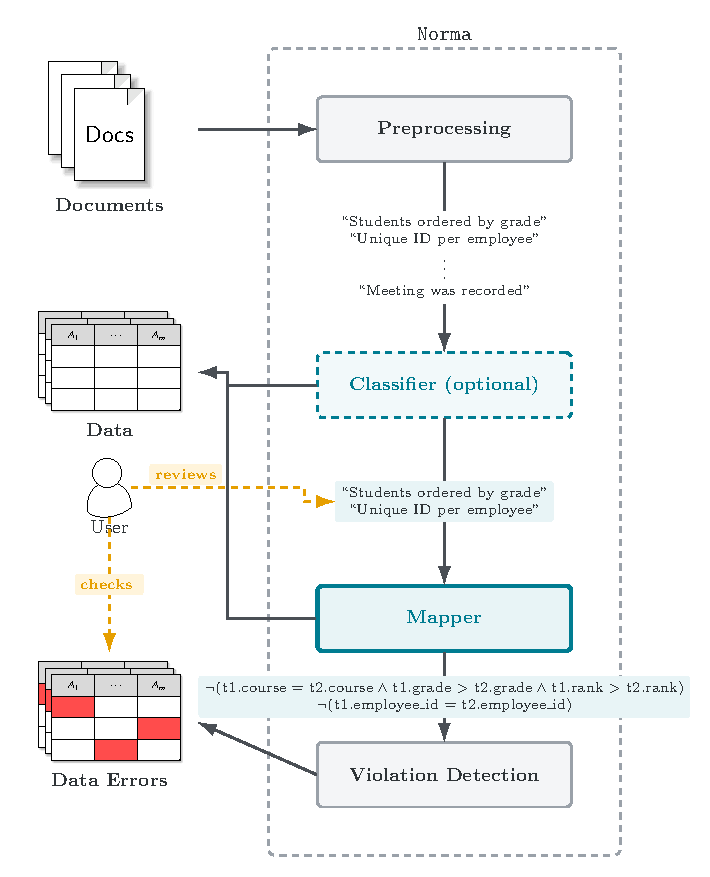
\includegraphics[width=0.85\columnwidth]{diagramas/pipeline_norma.pdf}
%\caption{The \system\ pipeline.}
\vspace{-10pt}
\caption{Overview of the \system\ pipeline. Blue components represent the novel contributions presented in this paper.}
\label{fig:pipeline}
\vspace{-10pt}
\end{figure}

\smallskip\noindent\textbf{Preprocessing.}
An automated pipeline converts documents (e.g., PDF files) into normalized text: it extracts the text, removes hyphenation, normalizes whitespace, and segments sentences, followed by minimal manual cleanup. We treat this step as input preparation.


\smallskip\noindent\textbf{Constraint classifier.}
Given the sentences from preprocessing, a lightweight classifier can optionally identify those that likely express checkable constraints, filtering out content that is clearly unrelated to data quality constraints.  Since constraints missed at this stage cannot be recovered downstream, we prioritize recall at this stage. False positives can still be ruled out by the mapper (which we define next). The classifier only labels the given sentences and never generates text, so it preserves the link between each sentence and its constraint. When no classifier is used, all sentences are passed directly to the mapper. A user can optionally be involved at this stage, reviewing and correcting the set of classified sentences before proceeding to mapping. We describe the classifier details in Section~\ref{sec:classifier}.


\smallskip\noindent\textbf{Constraint mapper.}
The mapper is the central and most complex component of \system. It takes each sentence, optionally pre-filtered by the classifier, and produces denial constraints grounded in the dataset schema.
It must interpret the sentence, align it with schema elements, and synthesize a constraint with correct violation semantics. Outputs that fail validation are rejected, and sentences that yield no valid constraint are excluded (Section~\ref{sec:mapper}).


\smallskip\noindent\textbf{Violation detection.}
Each constraint is validated by compiling it into a SQL violation query and executing it on the target relation (Section~\ref{sec:mapper:sql}), and it is linked back to the sentence that produced it. \system\ returns the violating tuples to the user for further inspection. DC violation detection is a well-studied problem, with specialized systems available for large-scale consistency checks~\cite{facet2021,liu2024rapidash,youri2024}. We compile DCs into SQL because the queries run on any engine that holds the data and also serve the data-based checks of the mapper; specialized engines can replace this step for larger workloads.



\section{Constraint Classification}
\label{sec:classifier}
Given the sentences $\mathcal{S}$ of a regulatory document (Section~\ref{sec:problem}), the constraint classifier aims at identifying the subset $\mathcal{S}_c \subseteq \mathcal{S}$ of sentences that state data quality constraints. A sentence is a positive example if it expresses a condition that the data is expected to satisfy and that can be 
validated against a dataset. Many sentences only define terms, describe procedures, or provide context. Constraint-related sentences appear less often, and many sentences that sound like rules are still too vague to test with data. 




\begin{example}[Restaurant inspections]
\label{ex:classification}
The NYC Department of Health publishes restaurant inspection results, 
including scores and letter grades,\footnote{Dataset available at 
\url{https://data.cityofnewyork.us/Health/DOHMH-New-York-City-Restaurant-Inspection-Results/43nn-pn8j}. See Section~\ref{sec:experiments} for details.} alongside a document 
describing the grading and inspection regulations.\footnote{Available at 
\url{https://www.nyc.gov/site/doh/services/restaurant-grades.page}.} 
The first two of the following sentences from these regulations state checkable rules, whereas the last two do not: ``A score of 0--13 results in a grade of A''; ``Every food service establishment is scheduled for at least one inspection per year''; ``Only certain inspections result in a grade'', which is too underspecified to test; and ``Consumers may check an establishment's inspection history'', which describes a user permission rather than a condition on the data.
\qed
\end{example}
%\vspace{-1cm}

%At this stage, we prioritize recall over precision: missed rules cannot be recovered downstream, while false positives can still be filtered by the constraint mapper. \system\ treats the classifier as a replaceable module that outputs binary labels or confidence scores. This modularity allows implementations to be swapped for cost, accuracy, or domain considerations. \system\ currently supports two types of classifier implementations.


%% use this if we include the SLM classifier
%At this stage, we prioritize recall over precision: missed rules cannot be recovered downstream, while false positives can still be filtered by the constraint mapper. \system\ treats the classifier as a replaceable module that outputs binary labels or confidence scores. This modularity allows implementations to be swapped for cost, accuracy, or domain considerations. \system\ currently supports two types of classifier implementations: \emph{LLM-based prompting} and \emph{fine-tuned encoders}. The LLM is more flexible and can incorporate schema and data samples at inference time, generalizing better out-of-domain but incurring API costs. The fine-tuned model is faster and cheaper but depends on training data diversity. Section~\ref{sec:experiments} quantifies these trade-offs.
    
%At this stage, we prioritize recall over precision: missed rules cannot be recovered downstream, while false positives can still be filtered by the constraint mapper. 
\system\ implements the classifier by prompting an LLM, which can incorporate schema and data samples at inference time and needs no labeled training data.

%\smallskip\noindent\textbf{LLM-Based Classification}
%\subsection{LLM-Based Classification}
\subsection*{Constraint Classification by Example}
%\label{sec:classifier:llm}
%We prompt large language models to label each sentence as stating a data quality rule or not. Figure~\ref{fig:classifyprompt} shows the prompt structure (full prompts are in the supplementary material). We use prompt variants that optionally include generic template examples and schema context (table description, columns, and sample tuples). We require structured output and parse responses with regular expressions; if parsing fails after retries, we default to non-constraint. Section~\ref{sec:experiments} evaluates closed- and open-weight models under these variants.

The model labels each sentence as stating a data quality rule or not; Figure~\ref{fig:classifyprompt} shows the prompt structure. 
%In our setting, some prompt variations include generic template examples and schema context, such as table descriptions, columns, and sample tuples.

%In our setting, labeled sentence templates, schema information, and sample tuples guide the model's labeling decisions across a large and heterogeneous sentence space. 
Each prompt carries a batch of up to 10 numbered sentences, and the model returns one label per sentence through a JSON schema. Malformed outputs are retried, then the sentences of the batch are classified one at a time, and a sentence that still has no valid label is marked as non-constraint. Section~\ref{sec:experiments} compares several models and the prompt variants described below.


\begin{figure}[!ht]
\centering
\footnotesize
\begin{tabularx}{\linewidth}{p{0.15\linewidth}X}
\toprule
\textbf{Task Definition} &
\hlc[neutralbg]{For each sentence, decide whether it states a DATA QUALITY CONSTRAINT that can be validated from the dataset when the required fields are available.}\\
\midrule

\textbf{Rule Types} &
%\hlc[neutralbg]{YES: includes:} \newline
\hlc[yesbg]{Required/non-null field; Allowed or forbidden values; Numeric bounds; Conditional requirements; Cross-row consistency; Determinacy; Temporal constraints; \ldots} \\
\midrule

\textbf{Exclusions} &
%\hlc[neutralbg]{NO: includes:} \newline
\hlc[nobg]{Headings, titles, citations; Definitions or descriptions; Procedures or human decisions; Statements not testable from the dataset; \ldots} \\
\midrule

\textbf{Examples} \newline \textit{(optional)} &
\hlc[neutralbg]{YES:} \newline
\hlc[yesbg]{``Field X is required.''} \newline
\hlc[yesbg]{``Two rows with the same Key must not disagree on Field H.''} \newline
\hlc[yesbg]{\ldots} \newline
\hlc[neutralbg]{NO:} \newline
\hlc[nobg]{``Field X represents the total amount.''} \newline
\hlc[nobg]{\ldots} \\
\midrule

\textbf{Context} \newline \textit{(optional)} &
%\hlc[neutralbg]{Table:} \hlc[contextbg]{[\textsf{Table Description}]} \newline
\hlc[neutralbg]{Table Schema:} \hlc[contextbg]{[\textsf{Column Names / Types}]} \newline
\hlc[neutralbg]{Table Sample Rows:} \hlc[contextbg]{[\textsf{Example Tuples}]} \\
\bottomrule
\end{tabularx}

\vspace{-0.3cm}
\caption{Constraint classification prompt structure (simplified).
Colors indicate: \csquare{yesbg}\,positive label clues, \csquare{nobg}\,negative label clues, \csquare{contextbg}\,data context, and \csquare{neutralbg}\,instructions.}
\vspace{-0.3cm}
\label{fig:classifyprompt}
\end{figure}


%\smallskip\noindent\textbf{Prompt structure.} Following standard practice in prompt-based text classification~\cite{sun2023textclassification}, we include a task definition, category descriptors, and optional labeled examples. 
%We find this strategies important, as constraint classification presents two challenges. First, the positive class is rare and heterogeneous, with many syntactic forms. We enumerate rule types to reduce false negatives; otherwise, models may miss constraints such as functional dependencies, where a key (or key-like attribute set) determines another attribute (e.g., two rows with the same key must agree on a field), and other cross-row consistency conditions.
%Second, the negative class is easily confused with constraints. Definitions, procedures, and contextual statements often use similar wording, refer to data-related terms, or include keywords that suggest a requirement. We list exclusions and add notes for common edge cases.

\smallskip\noindent\textbf{Prompt structure.}
Following standard practice in prompt-based text classification~\cite{sun2023textclassification}, the prompt has a task definition, category descriptors, and examples, which address two challenges. First, the positive class is rare and spans many syntactic forms, so we enumerate the rule types to treat as constraints; otherwise, the model may miss, e.g., functional dependencies stated in specific language. 
%We also include examples of cross-row consistency conditions. 
Second, non-constraint sentences are easily mistaken for constraints. Definitions, procedures, and contextual statements often use similar wording, mention data-related concepts, or contain keywords that suggest a requirement. To reduce this confusion, we list exclusions and add notes on edge cases (omitted in Figure~\ref{fig:classifyprompt}).

\smallskip\noindent\textbf{Examples.} Following few-shot in-context learning~\cite{brown2020language}, the prompt includes a few task examples. They are generic templates that remain fixed across datasets rather than domain-specific examples, so the prompt remains portable without labeled data.

%To further illustrate this, in Section~\ref{sec:experiments}, we evaluate the impact of examples on recall.



\smallskip\noindent\textbf{Table Context.}
Prompt variants may also provide table context: column information and sample tuples. Schema context helps reject sentences that cannot be checked against the available fields, mainly improving precision, but it lengthens the prompt and makes predictions sensitive to the sample tuples.












%\subsection{Fine-Tuned Classifier}
%\label{sec:classifier:finetuned}
%
%Prompting an LLM for each sentence can be expensive for long documents. As a lower-cost alternative, we finetune a pretrained encoder to screen sentences before the mapping stage. Constraint classification can be viewed as a binary text classification problem: given a sentence, predict whether it states a data quality rule.
%
%\smallskip\noindent\textbf{Pretrained encoders for text classification.}
%Text classification with pretrained language models is well studied~\cite{plmClassification2025}. We follow the standard finetuning approach based on BERT~\cite{devlin-etal-2019-bert}: a pretrained encoder produces a sentence representation, and a lightweight classification head predicts the binary label. Finetuning pretrained encoders is a common transfer learning approach for natural language classification tasks and typically performs well even with limited labeled data~\cite{gururangan-etal-2020-dont}. Several encoder variants are available, including general-domain BERT-style models and domain-specific models such as Legal-BERT~\cite{chalkidis-etal-2020-legal} for legal text. We evaluate multiple variants in Section~\ref{sec:experiments}.
%
%In this implementation, we use sentence-only input to keep the classifier fast and compatible with smaller encoder models that have a limited maximum input length (in tokens). Joint text-and-schema encoding is possible for table-related tasks~\cite{TURL2022}, but we leave schema-aware encoders for this type of classifier as future work. Schema context is still supported in the LLM-based classifier.
%
%
%\smallskip\noindent\textbf{Adapting to the constraint domain.}
%Pretrained encoders learn from broad textual corpora, but text on data rules represents a narrower linguistic domain with specific vocabulary and structure. Prior work shows that adapting language models to the target domain can improve downstream performance~\cite{gururangan-etal-2020-dont}. However, collecting training data for the data quality domain is difficult: the boundary between constraint and non-constraint sentences is subtle and requires high expertise, making large-scale annotation expensive. To address this, we propose generating synthetic training data using an LLM guided by explicit instructions that describe the constraint domain.
%
%\smallskip\noindent\textbf{Training data generation.}
%Recent work shows that LLM-generated data can approach real-world data for training text classifiers when the task is objective and well-defined~\cite{li-etal-2023-synthetic}. However, models trained on synthetic data can overfit to surface patterns if the generated examples lack diversity~\cite{data_augmentation2020}. We propose two complementary strategies to address this.
%
%\emph{Paraphrase augmentation} takes labeled sentences from other datasets and prompts the LLM to generate variants that preserve meaning while changing wording and structure. For each seed sentence, we generate multiple paraphrases, increasing lexical diversity within each constraint type and helping the classifier generalize beyond specific phrasings.
%
%\emph{Schema-grounded synthesis} prompts the LLM with the target schema (column names and sample tuples), labeled examples from other datasets, and a list of common rule patterns (required fields, allowed values, numeric bounds, cross-row consistency, determinacy).
%The LLM generates new sentences that reference actual column names from the target schema. This increases coverage across constraint types relevant to the target dataset. We apply the same setup to synthesize non-constraint sentences, targeting definitions, procedures, and contextual statements that cover difficult negatives.
%
%
%Note that we exclude labeled sentences from the target document from training, and schema information is used only to guide the LLM during generation. This makes the approach portable as a fine-tuned classifier can be trained for any new dataset without manual annotation.
%
%
%%Together, paraphrases increase variation within observed rule types, while schema-grounded synthesis increases coverage across rule patterns tied to the schema.
%
%
%\smallskip\noindent\textbf{Training.}
%Constraint sentences are rare in regulatory documents, creating class imbalance that biases the model toward predicting non-constraint. We oversample constraint sentences and apply focal loss~\cite{focalLoss2020}, which down-weights easy negatives and focuses training on difficult examples such as non-constraints that resemble rules.
%Since lower encoder layers capture general linguistic patterns and upper layers are task-specific~\cite{rogers-etal-2020-primer}, we use layerwise learning rate decay to preserve pretrained knowledge in lower layers while allowing upper layers to adapt. Training details are in the supplementary material.
%
%
%\smallskip\noindent\textbf{Threshold selection.}
%The classifier outputs a probability $P(\text{constraint} \mid s)$ for each sentence. A threshold of 0.5 maximizes accuracy, but since missed constraints cannot be recovered downstream, we tune the threshold on a validation set to achieve recall of at least 0.85 while maximizing precision.

\section{Constraint Mapping}
\label{sec:mapper}

Let $\mathcal{S}$ denote the sentences passed to the mapper, either all preprocessed sentences or the subset retained by the classifier. For each $s_i \in \mathcal{S}$, the mapper returns a constraint $\varphi_i$ over the dataset schema, made of one or more DCs of the form $\neg(p_1 \land \cdots \land p_\ell)$ (Section~\ref{sec:mapper:sql}), or no output if $s_i$ does not express a constraint or cannot be linked to the schema. The task is to interpret the sentence, identify the relevant schema elements, select predicates that capture the rule, and produce an executable \emph{violation condition}. It is related to Text-to-SQL~\cite{yu2018spider}, but Text-to-SQL retrieves satisfying records, whereas our target is a conjunction of predicates that identifies a violation.

For instance, the rule ``A score of 0--13 results in a grade of A'' (Example~\ref{ex:classification}) has the violation condition
$\texttt{t.score} \geq \texttt{0} \land \texttt{t.score} \leq \texttt{13} \land \texttt{t.grade} \neq \texttt{`A'}$: any tuple satisfying all three predicates violates the rule.

A rule may be phrased in many ways, often with implicit references to schema elements, literals, or tuple relationships. We therefore rely on LLMs, motivated by their performance in Text-to-SQL~\cite{llmTEXT2SQLSurvey2025}. Unrestricted generation, however, is unreliable: LLMs are known to hallucinate column names and use unsupported operators~\cite{dail2025,llmTEXT2SQLSurvey2025,DBLP:conf/dexa/DociniAO25}, and we observed that they tend to describe valid states rather than violations. Our design follows two principles. First, a \emph{predicate space} derived from the schema serves as a controlled vocabulary: the mapper selects predicates from it or instantiates typed placeholders of predefined templates. Second, the mapper is biased toward \emph{precision}: an incorrect mapping produces false violations, whereas an unmapped sentence can still be inspected manually. We implement two mappers over the same predicate space, a \emph{single-prompt} mapper (Section~\ref{sec:mapper:llm}) and a \emph{multi-step} mapper (Section~\ref{sec:mapper:multistep}); both produce DCs that are compiled into SQL violation queries (Section~\ref{sec:mapper:sql}).

\subsection{Predicate Space}
\label{sec:mapper:predicate-space}

DC discovery operates over a \emph{predicate space}, the set of predicates allowed in candidate constraints~\cite{chu2013discovering,Pena2019DiscoveryDC}. Because discovery enumerates combinations of predicates, this space is kept small. Regulatory text, however, frequently refers to enumerations, ranges, string formats, and arithmetic conditions. Comparisons with constants and null checks are expressible as DCs, but discovery spaces rarely include set membership, patterns, or arithmetic, because each extension multiplies the candidates to enumerate. \system\ does not enumerate candidates; it uses the larger space only as a controlled vocabulary, which avoids candidate explosion while preserving syntactic validity.

\smallskip\noindent\textbf{Predicate templates.}
We derive the following categories from the schema:
(1)~\emph{cross-tuple} predicates (e.g., \texttt{t1.A = t2.A}), with $\{=,\neq\}$ for type-compatible attributes and also $\{<,\leq,>,\geq\}$ for numeric ones;
(2)~\emph{same-tuple} predicates (e.g., \texttt{t1.A $\leq$ t1.B});
(3)~\emph{null} predicates (\texttt{IS [NOT] NULL});
(4)~\emph{attribute--constant} predicates (e.g., \texttt{t1.A $\geq$ c});
(5)~\emph{pattern} predicates (\texttt{t1.A LIKE p});
(6)~\emph{set} predicates (\texttt{t1.A IN C}); and
(7)~\emph{arithmetic} predicates over numeric attributes of the same tuple (e.g., \texttt{t1.A $\geq$ c * t1.B}).
For categories 4--7, the mapper instantiates $c$, $p$, or $C$ with literals from the sentence. Following DC discovery~\cite{chu2013discovering}, order predicates are generated only for numeric attributes, and two-attribute predicates only for type-compatible pairs with overlapping values.

\smallskip\noindent\textbf{Coverage and scope.}
Across our six datasets, 487 of the 490 predicates of the gold DCs belong to this space; the three exceptions, on HMDA Checks, compare an integer-encoded date with arithmetic over the reporting year. The space excludes aggregation and arithmetic over dates or sequences of records, so rules over counts or inspection histories require derived attributes (Section~\ref{sec:datasets}). The target is a DC with at most two tuple variables and universal violation semantics: a single violating pair suffices. Rules that must hold only for most pairs, or that compare distances between values, such as differential dependencies, require counting or tolerance semantics and are outside our scope.

\smallskip\noindent\textbf{Schema-driven, on-demand generation.}
With arithmetic and code-set templates, the space of a 135-column table reaches hundreds of thousands of templates, most irrelevant to any given sentence. \system\ therefore stores only a \emph{schema description}: for each column, its type, admitted operators, domain values (when it has few distinct values), and a short description written offline by an LLM from a deterministic data profile, merged with the official data dictionary when available (HMDAZ). Once the relevant columns of a sentence are selected, predicates are generated only for them. For a fixed instance, the generated set equals the full space restricted to those columns, so the vocabulary is unchanged; only its materialization is deferred.

\subsection{Single-Prompt Mapper}
\label{sec:mapper:llm}

The single-prompt mapper performs the full mapping in one LLM call for a batch of three sentences. The prompt contains the definition of a DC, a small set of examples covering thresholds, set membership, field comparisons, nulls, cross-tuple rules, and non-constraints, and the columns retrieved for the batch: columns are ranked by the embedding similarity between the sentence and the column name and description, and the prompt carries the description, domain values, and generated predicates of each retrieved column. For each sentence, the model returns a list of independent rules, whose violations are united (Section~\ref{sec:mapper:sql}), or \texttt{null} if the sentence is not mappable.

\smallskip\noindent\textbf{Violation form.}
Without explicit guidance, LLMs tend to output predicates describing \emph{satisfying} tuples rather than \emph{violating} ones, since regulatory sentences describe what must hold. For the score rule above, the correct output is \texttt{grade $\neq$ `A'}, not \texttt{grade $=$ `A'}. The prompt states the criterion explicitly (``must be X'' $\Rightarrow$ \texttt{!= X}; ``must not be X'' $\Rightarrow$ \texttt{= X}), and the model must first state the condition under which a tuple violates the rule (\texttt{violated\_when}) before writing the DC.

\smallskip\noindent\textbf{Cross-tuple constraints.}
For rules that relate records, the mapper must introduce two tuple aliases and a join on the shared identifier; cues such as ``for the same'' or ``repeated'' in the prompt suffice for the model to generalize to other phrasings.

\smallskip\noindent\textbf{Literal grounding.}
A recurring failure is to produce thresholds, strings, or enumerations in the wrong format or casing. The domain values of each retrieved column anchor literals to the data representation (e.g., a label such as \texttt{'Secured by a first lien'} rather than a paraphrase).

\smallskip\noindent\textbf{Validation.}
Every predicate must reference existing columns, use admitted operators and typed constants, and have no placeholders. Malformed outputs are retried, invalid rules are returned once to the model with the error, and a sentence whose attempts all fail produces no constraint. Membership in the predicate space is not enforced; we report out-of-space predicates instead.

\subsection{Multi-Step Mapper}
\label{sec:mapper:multistep}

A single prompt must solve schema linking, predicate selection, literal grounding, and the violation form jointly, so early errors propagate: a wrong column breaks predicate selection, a hallucinated literal yields a valid but meaningless DC, and a non-constraint triggers an unnecessary mapping. In Text-to-SQL, separating schema linking from later decisions often improves accuracy~\cite{DBLP:conf/dexa/DociniAO25,redsql2025,dail2025,resdsql2023}. The multi-step mapper uses four LLM calls, each receiving the output of the previous one (Figure~\ref{fig:multistepprompt}), followed by deterministic checks. Each stage isolates one decision that the single-prompt mapper makes jointly, trading additional calls for smaller decisions that can each be validated. In our experiments, this decomposition keeps the mapper usable with backbones whose single-prompt outputs fail (Section~\ref{sec:constraintextraction}); a finer ablation that removes or reorders individual stages is left for future work.

\begin{figure}[!ht]
\centering
\footnotesize
\begin{tabularx}{\linewidth}{p{0.17\linewidth}p{0.26\linewidth}X}
\toprule
\textbf{Step} & \textbf{Context} & \textbf{Task} \\
\midrule
\textbf{Schema} &
\hlc[contextbg]{Schema description} &
\hlc[neutralbg]{Identify all columns relevant to $s$: direct mentions, synonyms, and derived concepts.}
\hlc[nobg]{Abort if no concept maps to a column.} \\
\midrule
\textbf{Predicates} &
\hlc[contextbg]{$\hookrightarrow$ Selected columns and their predicates} &
\hlc[neutralbg]{Select predicates and templates and the constraint pattern (value mapping, temporal bound, dependency, required field, conditional rule).}
\hlc[nobg]{Abort if none fits.} \\
\midrule
\textbf{Rule filter} &
\hlc[contextbg]{$\hookrightarrow$ Columns and predicates} &
\hlc[neutralbg]{Decide whether $s$ is a specific rule verifiable from column values alone.} \newline
\hlc[nobg]{Reject: processes, permissions, vague quantifiers.} \\
\midrule
\textbf{Construction} &
\hlc[contextbg]{$\hookrightarrow$ Selected predicates, column profiles} &
\hlc[neutralbg]{Instantiate placeholders with literals from $s$ and return the DC in violation form.} \\
\bottomrule
\end{tabularx}
\caption{Prompt structure of the multi-step mapper; context narrows progressively.
\csquare{contextbg}\,input context;
\csquare{nobg}\,abort\,/\,reject signal;
\csquare{neutralbg}\,instruction.}
\label{fig:multistepprompt}
\end{figure}

\smallskip\noindent\textbf{Stages.}
\emph{Schema linking} identifies the columns relevant to the sentence, including implicit references, and rejects the sentence if none applies. \emph{Predicate selection} chooses, among the predicates generated for those columns, the ones that together form the DC pattern; a dedicated structural step improves accuracy in Text-to-SQL~\cite{resdsql2023}. The \emph{rule filter} decides whether the sentence maps to a DC under the grounding obtained so far. Unlike the classifier (Section~\ref{sec:classifier}), it sees the candidate columns and predicates, and many sentences that look like rules in isolation support no executable constraint once grounded. Placing it before construction avoids a call for rejected sentences. \emph{Construction} instantiates the selected templates with thresholds, constants, patterns, and enumerations aligned with the data representation. Framing this step as grounded instantiation rather than open-ended generation makes unsupported predicates and malformed expressions less likely~\cite{pourreza2023din,picard2021,lin-etal-2020-bridging}.

\smallskip\noindent\textbf{Data-grounded checks.}
Each candidate DC is first validated structurally: predicates must belong to the predicate space, reference valid columns, use type-compatible operators, and contain no placeholders. Next, for each equality, string inequality, \texttt{LIKE}, or membership predicate with literals, we issue an existence query; a predicate that no tuple satisfies is an \emph{orphan predicate}, and a DC containing one is discarded. Numeric bounds and null predicates are exempt, since their validity is structural. Finally, we execute the DC and discard it when more than 90\% of the tuples take part in a violation: a DC that flags almost every tuple most likely encodes the valid state rather than its violation.

\subsection{From Denial Constraints to SQL}
\label{sec:mapper:sql}

Every DC is compiled into a SQL \emph{violation query}, used by the data-grounded checks, for violation detection, and for evaluation. Compilation is deterministic, but it settles questions that the DC formalism leaves open on real data.

\smallskip\noindent\textbf{Rule structure and compilation.}
Each rule is a tree of \texttt{AND}/\texttt{OR} nodes over the predicate forms of Section~\ref{sec:problem}; a rule with disjunctions is equivalent to one DC per disjunct of its disjunctive normal form. Independent rules of a sentence are compiled separately, and their violations are united. A rule with one tuple variable becomes a selection returning the identifiers of the violating tuples; a rule with two becomes a self-join with $t_1.\mathit{tid} \neq t_2.\mathit{tid}$. Membership and pattern predicates map to \texttt{IN} and \texttt{LIKE}, division is guarded against zero, and literals are canonicalized. The self-join condition must not be replaced by $t_1.\mathit{tid} < t_2.\mathit{tid}$, a common way to avoid reporting a pair twice: this is only correct for symmetric DCs, such as FDs. For the asymmetric ordering rule of Example~\ref{ex:intro}, it misses every pair whose witnesses appear in the opposite order (61 applications flagged with $\neq$, only 9 with $<$). Since violations are reported per tuple, enumerating both orders does not inflate the counts.

\smallskip\noindent\textbf{Types, missing values, and execution.}
Published data rarely matches its declared schema; numeric fields contain codes such as \texttt{NA} or \texttt{Exempt}. We read the data as text, type each column with the schema, and compare numeric attributes through \texttt{TRY\_CAST}, which turns malformed values into \texttt{NULL} instead of aborting the query. Under three-valued logic, a predicate over \texttt{NULL} is unknown and the tuple is not reported, so requiredness must be stated with \texttt{IS NULL}, and \texttt{loan\_type != 1} silently skips tuples without a loan type; the prompts illustrate this explicitly. Queries run on DuckDB under a memory budget, a time limit, and a result cap, since a pair DC that joins on a low-cardinality attribute can produce billions of bindings. A query that exceeds them is reported as an execution error, never as a constraint without violations.

\smallskip\noindent\textbf{Bridging text and data.}
Most of the difficulty lies before compilation, in the inferences that make the query check what the text means (Table~\ref{tab:sql-examples}). On Tax, ``lower salary cannot have higher tax rate'' becomes an asymmetric pair DC. On SISU, ``selected in only one of their options'' requires identifying the student by the national ID rather than the exam registration number, which the text leaves implicit. On HMDA Checks, amounts are recorded in thousands, so ``\$1,000 (\$1 million)'' becomes \texttt{loan\_amount >= 1000}, and ``five times the income'' becomes an arithmetic predicate. On HMDAZ, the regulation compares the APR with the average prime offer rate, a difference stored as \texttt{rate\_spread}, and combines coverage conditions, alternative thresholds, and labels that must match the data verbatim. Each decision changes the violating tuples, which is why we report violation detection next to structural extraction.

\begin{table*}[t]
  \centering
  \caption{Gold constraints compiled into violation queries, with the number of violating tuples (HMDA: first 1M rows). Numeric attributes are compared through \texttt{TRY\_CAST}. The HMDAZ condition is abridged ($\ldots$). $^{\dagger}$Translated from Portuguese.}
  \label{tab:sql-examples}
  \footnotesize
  \setlength{\tabcolsep}{4pt}
  \begin{tabular}{>{\raggedright\arraybackslash}p{1.6cm}>{\raggedright\arraybackslash}p{4.6cm}>{\raggedright\arraybackslash}p{9.0cm}r}
    \toprule
    \textbf{Dataset} & \textbf{Sentence (abridged)} & \textbf{Violation condition in the compiled query (\texttt{WHERE} clause, casts omitted)} & \textbf{Viol.} \\
    \midrule
    Tax & Within the same state, a person with lower salary cannot have higher tax rate. & \texttt{t1.tid <> t2.tid AND t1.state = t2.state AND t1.salary < t2.salary AND t1.rate > t2.rate} & 363 \\
    SISU & The student will be selected in only one of their options.$^{\dagger}$ & \texttt{t1.tid <> t2.tid AND t1.cpf = t2.cpf AND t1.edicao = t2.edicao AND t1.ano = t2.ano AND t1.etapa = t2.etapa AND t1.opcao != t2.opcao AND t1.aprovado = 'S' AND t2.aprovado = 'S'} & 149 \\
    HMDA Checks & If loan amount and income are $>0$ and the loan amount is $\geq$ \$1,000 (\$1 million), then loan amount should be $<$ 5 times the income. & \texttt{t1.loan\_amount > 0 AND t1.applicant\_income > 0 AND t1.loan\_amount >= 1000 AND t1.loan\_amount >= (5 * t1.applicant\_income)} & 600 \\
    HMDAZ & A high-cost mortgage is a consumer credit transaction secured by the consumer's principal dwelling in which the APR exceeds the APOR by more than (A) 6.5 points for a first lien, (B) 8.5 points for a first lien on personal property under \$50,000, or (C) 8.5 points for a subordinate lien. & \texttt{t1.business\_or\_commercial\_purpose = 2 AND t1.occupancy\_type\_name = 'Principal residence' AND t1.reverse\_mortgage\_name = 'Not a reverse mortgage' AND t1.hoepa\_status\_name = 'Not a HOEPA loan' AND ((t1.lien\_status\_name = 'Secured by a first lien' AND (\ldots) AND t1.rate\_spread > 6.5) OR (\ldots\ \textrm{case (B)}) OR (t1.lien\_status\_name = 'Secured by a subordinate lien' AND t1.rate\_spread > 8.5))} & 4 \\
    \bottomrule
  \end{tabular}
  
\end{table*}

\subsection{Methodological Contributions}
\label{sec:mapper:novelty}

Two components of \system\ are adapted from Text-to-SQL practice~\cite{resdsql2023,pourreza2023din}: schema linking, which here operates over a schema description with column descriptions and domain values, and the staged decomposition, to which \system\ adds a rule filter that decides whether the text is a checkable rule at all, whereas every Text-to-SQL question has an answer. The remaining components are specific to Text-to-Constraints: the predicate space of typed templates derived from the schema and generated on demand; the violation form, which makes the output the condition that must never hold (a DC), a canonical target instead of a query; the data-grounded checks of orphan literals and of the share of violating tuples; the compilation, with its pair, type, and \texttt{NULL} semantics; and the evaluation, with equivalence-aware extraction, execution equivalence, and per-rule metrics (Section~\ref{sec:metrics}). Prompts implement individual decisions, but replacing a prompt changes neither the vocabulary, the violation form, nor the checks that every constraint must pass.




\section{Experimental Evaluation}
\label{sec:experiments}

Our evaluation of the \system\ prototype addresses four questions: \textbf{RQ1}, how accurately can \system\ identify the sentences that express data constraints? \textbf{RQ2}, how accurately can it map them to executable DCs that capture the corresponding violations? \textbf{RQ3}, how do classifier and mapper implementations, LLM backbones, and prompt variants affect quality and robustness? \textbf{RQ4}, how does \system\ compare with data profiling and Text-to-SQL baselines?

\subsection{Datasets}
\label{sec:datasets}

%No benchmark currently exists for the \emph{Text-to-Constraints} problem.
%We prepared four datasets for our experiments. Two are based on real-world regulatory documents paired with corresponding tabular datasets, and two are derived from datasets widely used in data quality and profiling research, for which the target constraints are already known. For the real-world datasets, we manually annotated the constraints expressed in the source text. For the derived datasets, we generated natural-language descriptions of the known constraints, as described below. When a constraint had no natural violations in the data, we injected a few violating records so that every constraint could be evaluated under the violation-based metrics of Section~\ref{sec:metrics}. 
%Table~\ref{tab:datasets} summarizes the datasets.


We evaluate \system\ on six datasets: four based on real-world regulatory documents paired with corresponding tabular datasets, and two derived from benchmark datasets commonly used in data quality and profiling research. Table~\ref{tab:datasets} summarizes them. For every dataset, the authors labeled each sentence and wrote its gold DC in violation form over the released schema; sentences not checkable on the released attributes are non-constraints. No sentence occurs twice, and near-identical sentences (similarity $\geq 0.9$) are templated statements that differ in one attribute or literal (13 pairs in SISU, 32 in HMDA Checks, at most two elsewhere), never sharing a gold DC.



\begin{table}[ht]
  \centering
  \caption{Dataset statistics. $^{\dagger}$First 1M rows of the public file (15.1M and 4.8M rows); \emph{Const.} counts sentences mapped to a non-null gold DC.}
  \label{tab:datasets}
\small
%  \resizebox{\columnwidth}{!}{%
  \begin{tabular}{lrrrrr}
    \toprule
    \textbf{Dataset} & \textbf{\#Rows} & \textbf{\#Cols} & \textbf{Sent.} & \textbf{Const.} & \textbf{Viol.} \\
    \midrule
    Hospital & 1k & 17 & 109 & 15 & 834 \\
    Restaurant & 128k & 21 & 33 & 7 & 52,311 \\
    SISU & 102k & 56 & 42 & 17 & 533 \\
    Tax & 100k & 15 & 126 & 6 & 468 \\
    HMDAZ$^{\dagger}$ & 1M & 135 & 17 & 9 & 209 \\
    HMDA Checks$^{\dagger}$ & 1M & 81 & 158 & 92 & 986,491 \\
    \bottomrule
  \end{tabular}%
  %}% resizebox
    
\end{table}

\smallskip\noindent\textbf{SISU.}
This dataset contains admission records of Brazil's university selection system (Example~\ref{ex:intro}). We annotated three sections of \textit{Portaria Normativa No.~21/2012} covering student
registration, candidate classification and selection, and waitlist procedures.
The constraints span 11 nullability checks, a functional dependency, an order dependency (Example~\ref{ex:intro}), a conditional functional dependency (a student is selected in at most one option), and three conditional DCs over one or two tuples. Many have violations in the released data.


\smallskip\noindent\textbf{Restaurant.}
This dataset pairs the NYC inspection records (Example~\ref{ex:classification}) with the grading and closure sections of the food service inspection guide, which constrain score-to-grade mappings, inspection frequency, grade posting, and closure conditions. For the one rule over inspection sequences, we added a derived column with the days until the next inspection; automating such transformations is future work.


\smallskip\noindent\textbf{Tax and Hospital.}
Both datasets are standard benchmarks in DC research~\cite{chu2013discovering,holoclean}, but their constraints exist only in formal form. An LLM (Claude~4.5 Sonnet, not evaluated in any \system\ configuration) wrote a description of each constraint and surrounding non-constraint sentences in schema terminology, mimicking a document that interleaves rules with other prose. These two datasets nevertheless form a controlled setting: their constraints come from prior papers and their sentences from an LLM that may share priors with the evaluated backbones, which likely makes them easier than real regulatory text. SISU, Restaurant, and the HMDA datasets, which pair real regulatory text with real data, are the more reliable signal.




\smallskip\noindent\textbf{HMDAZ and HMDA Checks.}
Both datasets use public loan-level records released under the Home Mortgage Disclosure Act (HMDA); we use the first 1M rows of each file. \emph{HMDAZ} pairs the 2018 loan application
register (135 columns, including the code and label versions of each
categorical field) with Sections 1026.32, 1026.35, and 1026.43 of Regulation~Z,
which define high-cost (HOEPA) and higher-priced mortgages, the limitations
that apply to them, and the ability-to-repay requirements. Sentences are verbatim from
the regulation, and gold DCs keep the coverage conditions of each trigger.
Scope-only text, or text whose outcome is not observable in the data, is
annotated with a \texttt{null} constraint. \emph{HMDA Checks} pairs the 2014
register (81 columns) with the 2014 HMDA edit specification published by the
FFIEC: one entry per edit, with the edit test verbatim; edits that cannot be
checked on a single record (aggregate, transmittal-sheet, or external-reference
edits) are \texttt{null}. Compared with the other datasets, these two add wide schemas whose relevant column is often named after a code rather than the concept in the text, rules with arithmetic, and highly concentrated violations.

\subsection{Baselines}
\label{sec:baselines}

Since no prior system addresses the Text-to-Constraints task directly, we compare \system\ against the two closest paradigms: DC discovery from data alone and Text-to-SQL.


\smallskip\noindent\textbf{Data profiling.}
We use the DC discovery algorithms from~\cite{Pena2022FastDC}, running both exact and approximate denial-constraint discovery. Exact DCs hold with no violations and thus cannot match rules violated in the data, so we focus on approximate DCs, which tolerate a fraction $\varepsilon$ of violating pairs. Since FDs and order dependencies with at most two tuples are special cases of DCs, approximate DC discovery over the same attributes subsumes their discovery, and we do not run separate FD or OD algorithms. Conditional variants require predicates with constants, which DC discovery supports only for a restricted set of values; a comparison with dedicated CFD discovery is left for future work.

We run exact discovery and $\varepsilon \in \{0.001, 0.005, 0.01, 0.05, 0.1\}$, rank the DCs by coverage and succinctness~\cite{chu2013discovering}, and report, for each metric, the best result over this grid and top-$k \in \{5, 10, 20, 50, 100\}$.

Since discovery does not scale to the full SISU, Restaurant, and HMDA schemas, we restrict them to the columns of the gold constraints, the most favorable setting for the baseline, and run it on a seeded sample of 100k of the 1M HMDA rows. On HMDA Checks (39 columns), no configuration finished: runs timed out or exhausted a 12\,GB heap even with samples of 10k rows.


\smallskip\noindent\textbf{Text-to-SQL.}
We prompt XiYan-SQL~\cite{XiYanSQL}, a state-of-the-art Text-to-SQL framework, to return for each sentence a query that selects the violating tuples, or \texttt{NULL} if the sentence is not a checkable constraint, so it acts as both classifier and mapper. We use the 32B model with three seeds and report the mean.


\subsection{Evaluation Metrics}
\label{sec:metrics}

We evaluate three dimensions; as in Text-to-SQL, execution-based evaluation complements structural matching, because exact form alone does not capture correctness~\cite{zhong-etal-2020-semantic}.
\emph{Constraint classification} measures precision, recall, and F$_1$ of the sentences labeled as constraints; it applies to \system\ and Text-to-SQL, not to profiling.
\emph{Constraint extraction} (CE) compares predicted and gold DCs by exact predicate-set match (precision, recall, F$_1$). For Text-to-SQL, predicates are read from the \texttt{WHERE} clause (a correlated \texttt{EXISTS} as a pair DC); a query with no DC reading, e.g., with aggregation or \texttt{CASE}, counts as correct if it returns exactly the violations of the gold DC.
\emph{Violation detection} executes all predicted and all gold constraints and compares the sets of tuples that take part in at least one violation (aggregate violation F$_1$, AV); it applies to all methods.

\smallskip\noindent\textbf{Complementary mapping metrics.}
Exact matching penalizes logically equivalent rewritings, and the tuple-level aggregate can be dominated by a single rule. We therefore also report:
(i)~\emph{equivalence-aware extraction} (CE$_{\equiv}$), which compares DCs after a logical normal form (e.g., \texttt{IN} as a disjunction, sorted operands) and unifies literals on a code column and its label column (e.g., \texttt{hoepa\_status = 1} and \texttt{hoepa\_status\_name = 'High-cost mortgage'}) only when the data confirms that they select the same tuples;
(ii)~\emph{execution equivalence}, the fraction of gold rules with violations whose predicted DC flags exactly the same tuples;
(iii)~\emph{per-rule violation F$_1$}, averaged over gold sentences so that every rule weighs the same; and
(iv)~\emph{violation concentration}, the share of gold-violating tuples flagged by the largest gold rule. Predicted DCs whose SQL fails are counted as errors, not as producing no violation.

\subsection{Implementation and Settings}
\label{sec:implementation}

\system\ is implemented in Python with DuckDB as the execution backend. All LLM calls go through OpenRouter with strict JSON-schema outputs. We evaluate six backbones: GPT-6 Luna, DeepSeek-V4-Flash, Mistral Large 4, Qwen3.8-2.4T-A95B, GPT-6 Sol, and Claude Sonnet 5.5. Kimi K2.6 (whitespace loops under strict decoding) and MiniMax-M3 (empty single-prompt outputs; Section~\ref{sec:constraintextraction}) were replaced. Classifier and mapper configurations run once, with up to 32k output tokens per call; end-to-end configurations run three times. A preliminary study with earlier backbones (e.g., Qwen3-32B and GPT-5) followed the same protocol on Hospital, Restaurant, SISU, and Tax; we refer to it in Section~\ref{sec:constraintextraction}. \system\ and DC discovery ran on a workstation with an Intel Core i7-7700HQ CPU and 16\,GB of memory, and XiYan-SQL on an NVIDIA A100 (80\,GB). The baselines are scored by the same evaluator, data, and query limits as \system.

\subsection{Classifier Performance}
\label{sec:constraintdetection}

Our first experiment evaluates how model and prompt design affect constraint classification. We derive four variants of the prompt in Figure~\ref{fig:classifyprompt} by enabling or disabling \emph{examples} and \emph{table context} (\emph{No Context}, \emph{Table Context}, \emph{Examples}, \emph{Examples + Table Context}) and evaluate them with six LLMs on all datasets (Figure~\ref{fig:classifier-results}). Because sentences missed here cannot be recovered by the mapper, we require recall $\geq 0.90$ on every dataset when selecting a default configuration.

\begin{figure}[!ht]
    \centering
    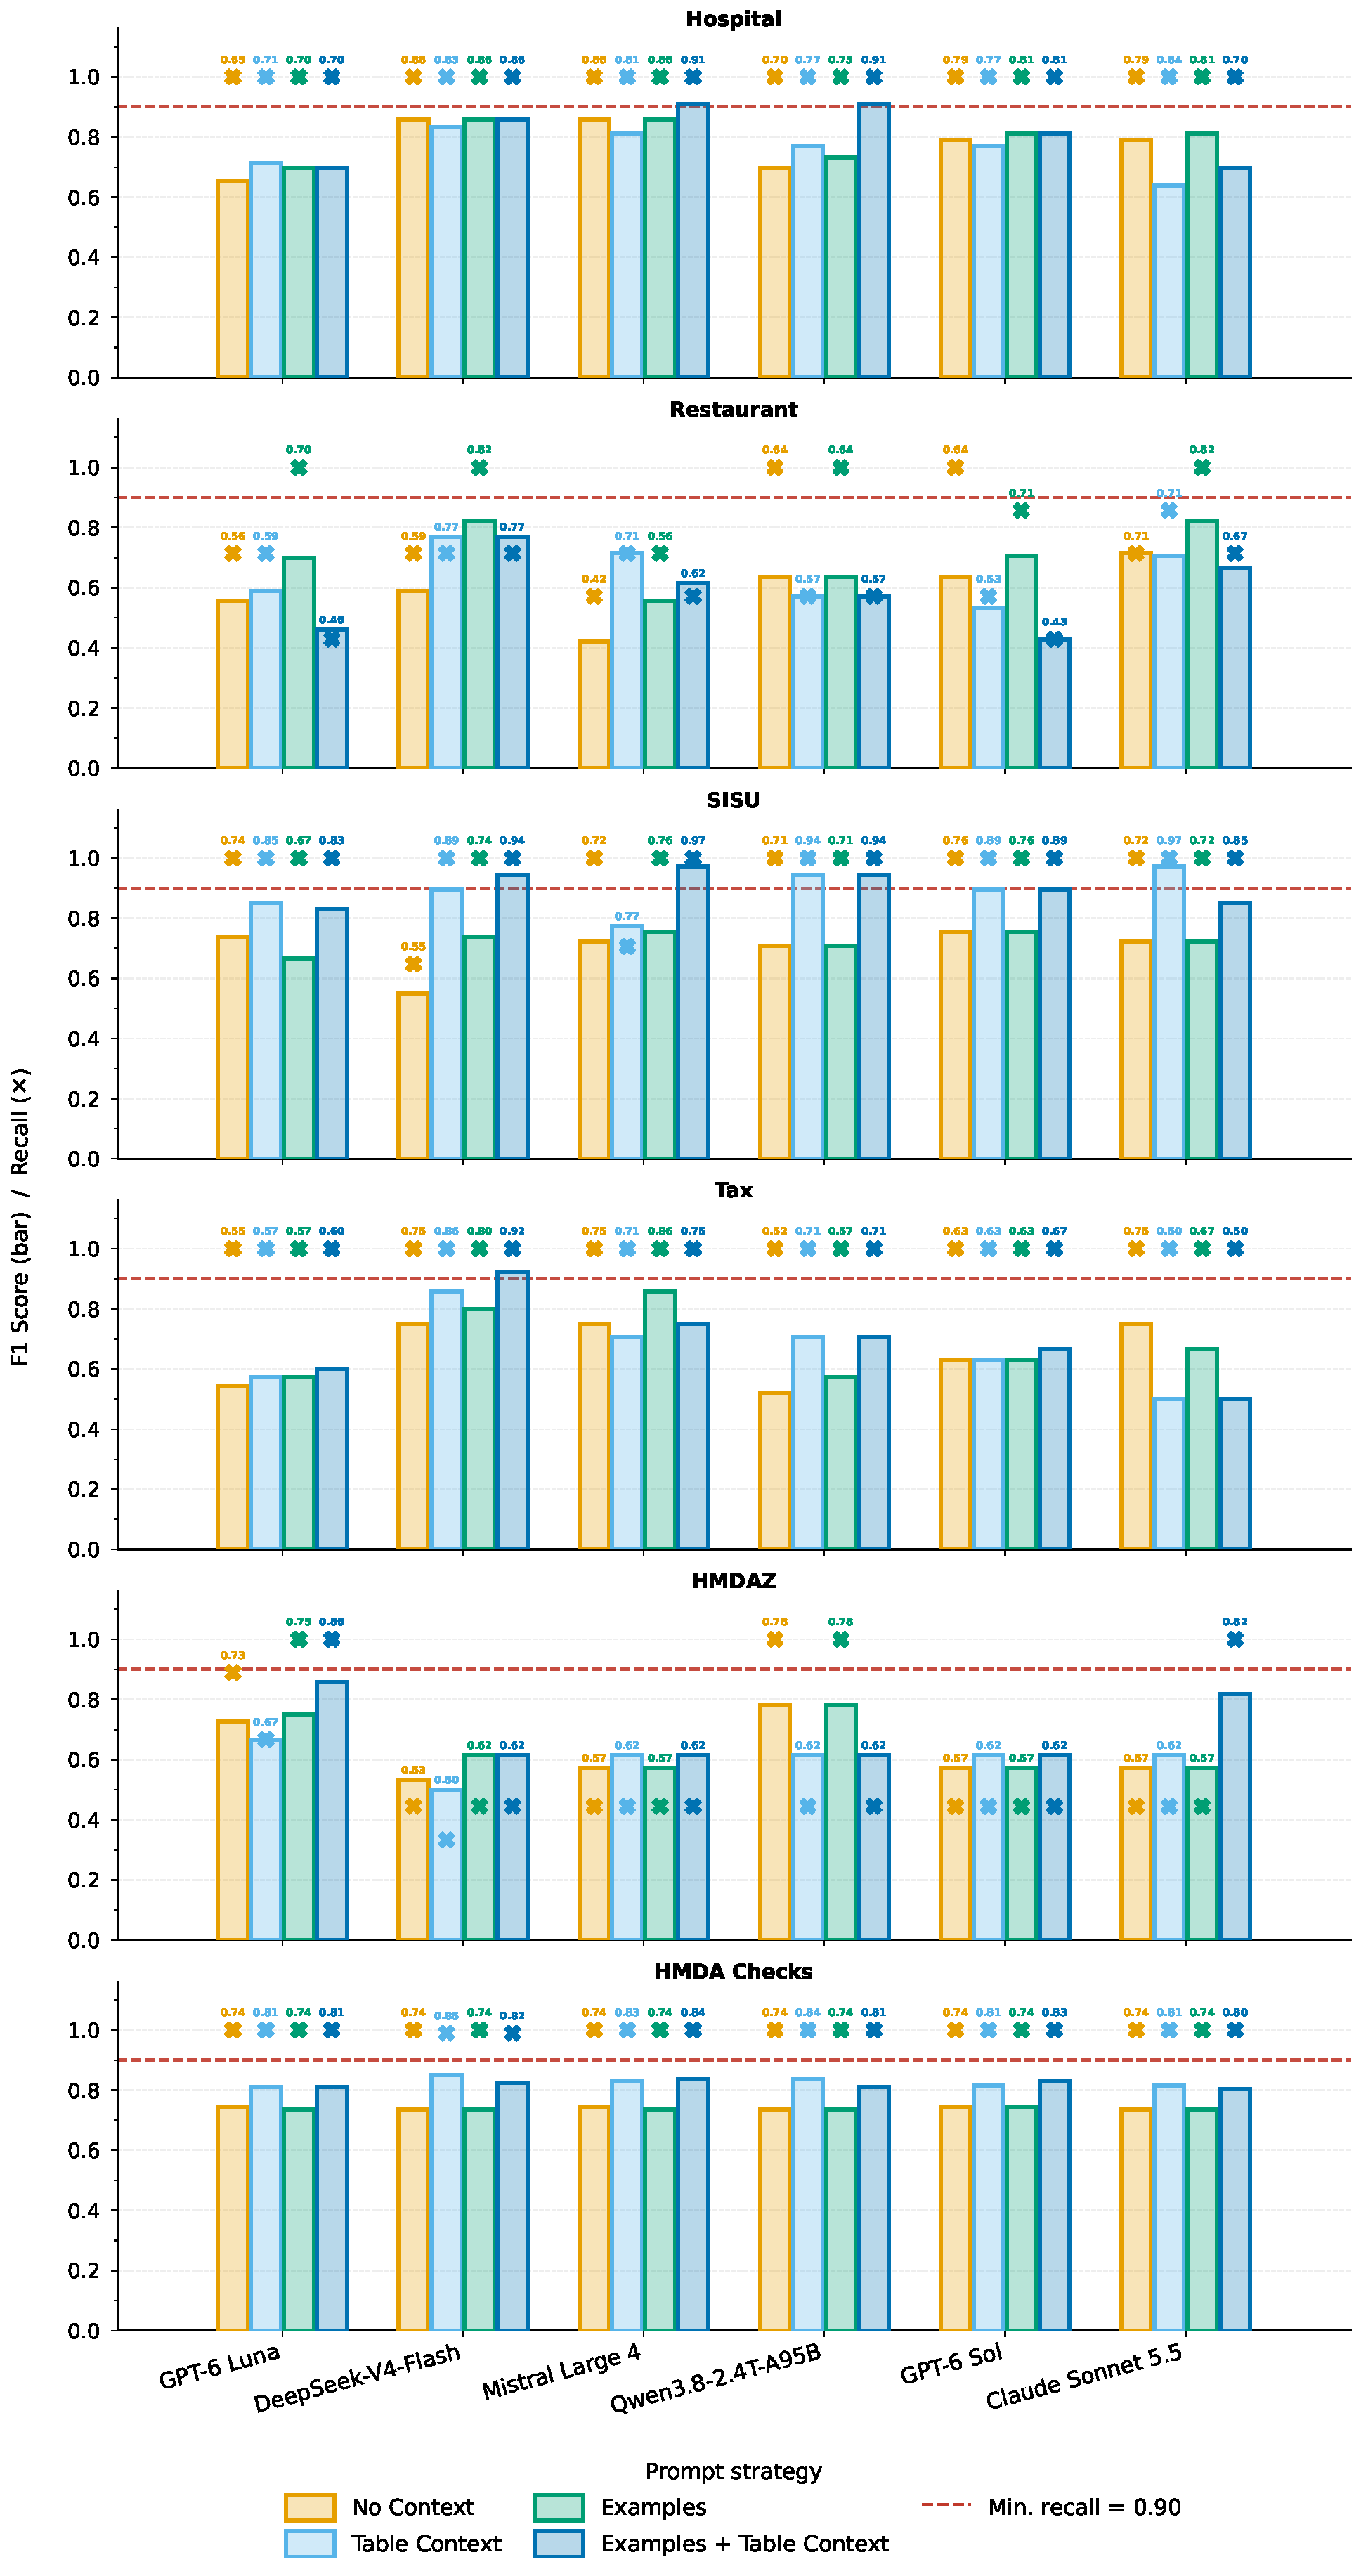
\includegraphics[width=0.85\columnwidth]{figures/results/v3_fig6_classifiers.pdf}
\caption{Constraint classification F$_1$ (bars) and recall (\textsf{x}) across models and prompt variants. The dashed line marks the 0.90 recall threshold.}
    \label{fig:classifier-results}
\end{figure}

On Hospital, Tax, SISU, and HMDA Checks, almost every configuration reaches recall 1.00, so differences lie in precision. On HMDAZ and Restaurant, recall is the bottleneck: on HMDAZ, most configurations recover only 4 of the 9 constraint sentences, missing regulatory definitions (e.g., when a mortgage is high-cost) that read as scope statements, although each implies a checkable condition. Only three configurations satisfy this recall requirement on all six datasets: \emph{Qwen3.8-2.4T-A95B} with \emph{Examples} (mean F$_1$ 0.69), \emph{GPT-6 Luna} with \emph{Examples} (0.69), and \emph{Qwen3.8-2.4T-A95B} with \emph{No Context} (0.68); we select the first. Configurations with higher mean F$_1$ exist (e.g., DeepSeek-V4-Flash with \emph{Examples + Table Context}, 0.82), but they miss more than half of the HMDAZ constraints.

Table context has two opposite effects. It is the only signal that raises precision on HMDA Checks, where non-constraint edits are phrased like checkable ones but refer to aggregates or external data: without it, F$_1$ equals that of the all-positive classifier (0.74); with it, 0.80--0.85. On wide schemas, however, it does not help recall: on HMDAZ (135 columns), 9 of the 12 table-context configurations stay at or below 0.44. Averaged over models and datasets, \emph{Examples} gives the best recall (0.93), and table context higher precision (0.71 vs.\ 0.58--0.62) at lower recall (0.85--0.87).
Without examples or context, classification is already strong on the controlled datasets (recall 1.00, mean F$_1$ 0.72 on Tax and Hospital), and the best variant adds only 0.04. On SISU, Restaurant, and the HMDA datasets, the gain is larger (0.66 to 0.75 with \emph{Examples + Table Context}), mostly through precision. A plausible explanation is that LLM-written sentences resemble text these models produce or saw in pretraining; we cannot verify such exposure, but context matters most on real regulatory text.

\subsection{Constraint Mapping Performance}
\label{sec:constraintextraction}

Our second experiment evaluates how model and mapper choices affect mapping quality. To isolate mapping from classification errors, we compute constraint extraction and aggregate violation F$_1$ on the ground-truth constraint sentences only, comparing the \emph{Single-Prompt} and \emph{Multi-Step} mappers with six LLMs (Figure~\ref{fig:mapper-results}, Table~\ref{tab:mapping-metrics}). On Hospital, Restaurant, SISU, and Tax, \emph{Multi-Step} improves both metrics (mean over models: 0.81 vs.\ 0.75 and 0.83 vs.\ 0.55), with the largest gains on Restaurant and SISU, whose rules combine several conditions or relate two tuples. The best Multi-Step configurations exceed the best one of the preliminary study (GPT-5, 0.78 and 0.95): Claude Sonnet 5.5 reaches 0.85 and 0.97, GPT-6 Luna 0.82 and 0.98, and Qwen3.8-2.4T-A95B 0.80 and 1.00. Decomposition also keeps the mapper usable with unstable backbones: MiniMax-M3 returned empty outputs for 107 of 156 Single-Prompt sentences but completed the Multi-Step pipeline without failures; among the final backbones, only DeepSeek-V4-Flash has output failures (3 Single-Prompt sentences).

\begin{figure}[!ht]
    \centering
    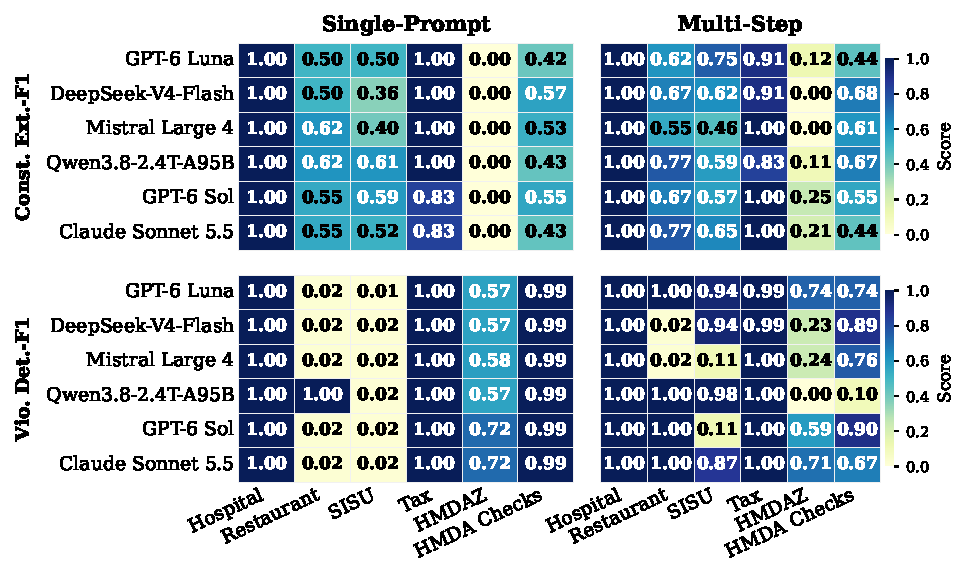
\includegraphics[width=0.85\columnwidth]{figures/results/v3_fig7_mapping.pdf}
    \caption{Sentence-level mapping results across models and mappers: constraint extraction F$_1$ and aggregate violation F$_1$ on ground-truth sentences.}
    \label{fig:mapper-results}
\end{figure}

\smallskip\noindent\textbf{Where Single-Prompt loses violations.}
On Restaurant, one rule (at least one inspection per year) flags 99\% of the gold-violating tuples. Every Single-Prompt configuration except Qwen3.8-2.4T-A95B returns \texttt{null} for it, so aggregate recall falls to 0.01; without this rule, all reach 1.00. On SISU, Single-Prompt identifies the student by the exam registration number instead of the national ID in the two-tuple rules, flagging about 51k tuples instead of 533. Multi-Step, which links columns and selects predicates before writing the DC, avoids both errors with most backbones, but not all: DeepSeek-V4-Flash and Mistral Large 4 also miss the Restaurant rule, and GPT-6 Sol and Mistral Large 4 make the identification error in one SISU rule (8.9k tuples; aggregate 0.11).

\begin{table}[!ht]
  \centering
  \caption{Mean mapping quality over the six datasets (ground-truth sentences). CE: exact extraction F$_1$; CE$_{\equiv}$: equivalence-aware extraction F$_1$; AV: aggregate violation F$_1$; Rule-F$_1$: mean per-rule violation F$_1$; Exec.: execution equivalence; Fail.: sentences with no valid output.}
  \label{tab:mapping-metrics}
  \small
  \setlength{\tabcolsep}{3.5pt}
  \resizebox{\columnwidth}{!}{\begin{tabular}{llrrrrrr}
\toprule
\textbf{Mapper} & \textbf{Model} & CM & CM$_{\equiv}$ & AV & Rule-F$_1$ & Exec. & Fail. \\
\midrule
\multirow{6}{*}{Single-Prompt} & GPT-6 Luna & 0.57 & 0.69 & 0.60 & 0.78 & 0.75 & 0 \\
 & DeepSeek-V4-Flash & 0.57 & 0.66 & 0.60 & 0.74 & 0.70 & 3 \\
 & Mistral Large 4 & 0.59 & 0.66 & 0.60 & 0.73 & 0.71 & 0 \\
 & Qwen3.8-2.4T-A95B & 0.61 & 0.70 & 0.76 & \textbf{0.86} & \textbf{0.83} & 0 \\
 & GPT-6 Sol & 0.59 & 0.67 & 0.62 & 0.76 & 0.72 & 0 \\
 & Claude Sonnet 5.5 & 0.55 & 0.64 & 0.62 & 0.76 & 0.70 & 0 \\
\midrule
\multirow{6}{*}{Multi-Step} & GPT-6 Luna & 0.64 & 0.69 & \textbf{0.90} & 0.77 & 0.76 & 0 \\
 & DeepSeek-V4-Flash & 0.65 & 0.69 & 0.68 & 0.68 & 0.69 & 0 \\
 & Mistral Large 4 & 0.60 & 0.64 & 0.52 & 0.74 & 0.73 & 0 \\
 & Qwen3.8-2.4T-A95B & 0.66 & 0.68 & 0.68 & 0.81 & 0.77 & 0 \\
 & GPT-6 Sol & 0.67 & 0.71 & 0.77 & 0.79 & 0.77 & 0 \\
 & Claude Sonnet 5.5 & \textbf{0.68} & \textbf{0.74} & 0.88 & 0.84 & 0.82 & 0 \\
\bottomrule
\end{tabular}
}
  
\end{table}

\smallskip\noindent\textbf{HMDA datasets.}
Exact extraction stays low (at most 0.25 on HMDAZ and 0.68 on HMDA Checks). Many predicted DCs are logically equivalent to the gold ones but written differently (\texttt{IN} instead of a disjunction, a label instead of its code column); others omit the coverage conditions of a trigger. Equivalence-aware extraction recovers much of the first group: on the HMDA datasets it raises mean extraction F$_1$ from 0.34 to 0.46 for Multi-Step and from 0.24 to 0.51 for Single-Prompt, while it barely changes elsewhere. On HMDA Checks, aggregate violation is not informative: two date-range edits flag 99\% of the gold-violating tuples, which cover 98.6\% of the rows, so a DC flagging every tuple already scores 0.99. Single-Prompt reaches 0.99 with every backbone, mostly through such DCs. Multi-Step scores 0.67--0.90 with five backbones, but only GPT-6 Sol maps a date edit correctly; the others write incorrect DCs for other edits that flag 480k--550k rows and pass the 90\% violation-share check. Without the two date edits, the Multi-Step aggregate falls to 0.12--0.19 for four backbones and stays at 0.98--1.00 for GPT-6 Sol and Qwen3.8-2.4T-A95B, while Single-Prompt ranges from 0.18 to 1.00. Per-rule metrics are far less sensitive: mean per-rule F$_1$ is 0.78 (Multi-Step) and 0.86 (Single-Prompt) with all edits, and 0.84 and 0.85 without the date edits.

\smallskip\noindent\textbf{Default mapper and sensitivity to the backbone.}
With Multi-Step, Claude Sonnet 5.5 has the best mean extraction (0.68) and GPT-6 Luna the best mean aggregate violation (0.90). The mean of the two selects \emph{Claude Sonnet 5.5} (0.776, against 0.771 for GPT-6 Luna and 0.720 for GPT-6 Sol), a tie with GPT-6 Luna given single runs. Backbones differ more in violation detection than in extraction: mean exact extraction ranges only from 0.60 to 0.68, aggregate violation from 0.52 to 0.90, and per-rule metrics lie in between (0.68--0.84). The divergences concentrate on implicit decisions rather than syntax: which attribute identifies an entity (SISU), whether a definition implies a checkable trigger (HMDAZ), and how integer-encoded dates are compared (HMDA Checks). Single runs also vary: two runs of Mistral Large 4 on Restaurant, differing only in a check unrelated to the dominant rule, scored 1.00 and 0.02 in aggregate because that rule was mapped in one run only. We cannot relate these differences to model size or training data, which most backbones do not disclose.

\subsection{End-to-End Evaluation and Comparison}
\label{sec:endtoend}

We evaluate the full pipeline with the default components, \emph{Qwen3.8-2.4T-A95B} with \emph{Examples} as classifier and \emph{Claude Sonnet 5.5} with \emph{Multi-Step} as mapper, in two variants: classifier plus mapper (C+MS) and the mapper alone, which relies on its rule filter (Multi-Step). Each variant runs three times, and Table~\ref{tab:main_results} reports the mean. Baseline results on Hospital, Restaurant, SISU, and Tax come from the preliminary study (Section~\ref{sec:implementation}), with the same data and gold constraints (their SISU violation scores predate the pair semantics of Section~\ref{sec:mapper:sql}); the baselines were not run on the HMDA datasets.

\begin{table}[!ht]
  \centering
  \caption{End-to-end comparison of \system\ (C+MS and Multi-Step; mean of three runs) and the baselines. \textbf{Profiling}: DC discovery from data alone; \textbf{Text2SQL}: XiYan-SQL adapted to generate violation queries; -- marks configurations not run; n/a, metric not applicable; bold, best F$_1$ per metric and dataset.}
  \label{tab:main_results}
  \small
  \setlength{\tabcolsep}{4pt}
  \resizebox{\columnwidth}{!}{%
  \begin{tabular}{llccccccccc}
\toprule
\textbf{Family} & \textbf{Method} & \multicolumn{3}{c}{Constr. Classification} & \multicolumn{3}{c}{Constr. Extraction} & \multicolumn{3}{c}{Viol. Detection} \\
\cmidrule(lr){3-5}  \cmidrule(lr){6-8}  \cmidrule(lr){9-11}
 &  & P & R & F$_1$ & P & R & F$_1$ & P & R & F$_1$ \\
\midrule
\addlinespace[2pt]
\multicolumn{11}{c}{\textbf{Hospital}} \\
\addlinespace[1pt]
\multirow{2}{*}{\system} & ~~C+MS & 0.81 & 1.00 & \textbf{0.89} & 1.00 & 1.00 & \textbf{1.00} & 1.00 & 1.00 & \textbf{1.00} \\
 & ~~Multi-Step & 0.48 & 1.00 & 0.65 & 1.00 & 1.00 & \textbf{1.00} & 1.00 & 1.00 & \textbf{1.00} \\
\cmidrule(l){2-11}
\multirow{1}{*}{Profiling} & ~~DC Discovery & n/a & n/a & n/a & 0.00 & 0.00 & 0.00 & 0.83 & 1.00 & 0.91 \\
\cmidrule(l){2-11}
\multirow{1}{*}{Text2SQL} & ~~XiYan-SQL & 0.50 & 1.00 & 0.67 & 0.60 & 1.00 & 0.75 & 0.83 & 1.00 & 0.91 \\
\midrule
\addlinespace[2pt]
\multicolumn{11}{c}{\textbf{Restaurant}} \\
\addlinespace[1pt]
\multirow{2}{*}{\system} & ~~C+MS & 0.89 & 0.71 & 0.79 & 0.80 & 0.57 & \textbf{0.67} & 1.00 & 0.34 & 0.35 \\
 & ~~Multi-Step & 0.65 & 0.71 & 0.68 & 0.80 & 0.57 & \textbf{0.67} & 0.87 & 0.01 & 0.02 \\
\cmidrule(l){2-11}
\multirow{1}{*}{Profiling} & ~~DC Discovery & n/a & n/a & n/a & 0.00 & 0.00 & 0.00 & 0.77 & 0.87 & \textbf{0.82} \\
\cmidrule(l){2-11}
\multirow{1}{*}{Text2SQL} & ~~XiYan-SQL & 0.86 & 0.75 & \textbf{0.80} & 0.17 & 0.12 & 0.14 & 0.45 & 0.64 & 0.52 \\
\midrule
\addlinespace[2pt]
\multicolumn{11}{c}{\textbf{SISU}} \\
\addlinespace[1pt]
\multirow{2}{*}{\system} & ~~C+MS & 0.67 & 1.00 & \textbf{0.80} & 0.65 & 0.65 & \textbf{0.65} & 0.03 & 0.98 & \textbf{0.06} \\
 & ~~Multi-Step & 0.65 & 1.00 & 0.79 & 0.65 & 0.65 & \textbf{0.65} & 0.03 & 0.97 & 0.05 \\
\cmidrule(l){2-11}
\multirow{1}{*}{Profiling} & ~~DC Discovery & n/a & n/a & n/a & 0.00 & 0.00 & 0.00 & 0.00 & 0.99 & 0.01 \\
\cmidrule(l){2-11}
\multirow{1}{*}{Text2SQL} & ~~XiYan-SQL & 1.00 & 0.65 & 0.79 & 0.45 & 0.29 & 0.36 & 0.00 & 1.00 & 0.01 \\
\midrule
\addlinespace[2pt]
\multicolumn{11}{c}{\textbf{Tax}} \\
\addlinespace[1pt]
\multirow{2}{*}{\system} & ~~C+MS & 0.71 & 1.00 & \textbf{0.82} & 1.00 & 1.00 & \textbf{1.00} & 0.59 & 1.00 & \textbf{0.70} \\
 & ~~Multi-Step & 0.33 & 1.00 & 0.50 & 1.00 & 1.00 & \textbf{1.00} & 0.01 & 1.00 & 0.02 \\
\cmidrule(l){2-11}
\multirow{1}{*}{Profiling} & ~~DC Discovery & n/a & n/a & n/a & 0.00 & 0.00 & 0.00 & 0.00 & 0.94 & 0.01 \\
\cmidrule(l){2-11}
\multirow{1}{*}{Text2SQL} & ~~XiYan-SQL & 0.40 & 1.00 & 0.57 & 0.29 & 0.67 & 0.40 & 0.01 & 1.00 & 0.02 \\
\midrule
\addlinespace[2pt]
\multicolumn{11}{c}{\textbf{HMDAZ}} \\
\addlinespace[1pt]
\multirow{2}{*}{\system} & ~~C+MS & 0.86 & 0.89 & 0.87 & 0.13 & 0.15 & 0.14 & 0.26 & 1.00 & 0.38 \\
 & ~~Multi-Step & 0.96 & 0.89 & \textbf{0.92} & 0.25 & 0.26 & \textbf{0.25} & 0.48 & 1.00 & \textbf{0.64} \\
\cmidrule(l){2-11}
\multirow{1}{*}{Profiling} & ~~DC Discovery & -- & -- & -- & -- & -- & -- & -- & -- & -- \\
\cmidrule(l){2-11}
\multirow{1}{*}{Text2SQL} & ~~XiYan-SQL & -- & -- & -- & -- & -- & -- & -- & -- & -- \\
\midrule
\addlinespace[2pt]
\multicolumn{11}{c}{\textbf{HMDA Checks}} \\
\addlinespace[1pt]
\multirow{2}{*}{\system} & ~~C+MS & 0.90 & 0.93 & 0.91 & 0.45 & 0.43 & 0.44 & 0.99 & 0.56 & \textbf{0.71} \\
 & ~~Multi-Step & 0.90 & 0.93 & \textbf{0.92} & 0.45 & 0.44 & \textbf{0.45} & 0.99 & 0.56 & \textbf{0.71} \\
\cmidrule(l){2-11}
\multirow{1}{*}{Profiling} & ~~DC Discovery & -- & -- & -- & -- & -- & -- & -- & -- & -- \\
\cmidrule(l){2-11}
\multirow{1}{*}{Text2SQL} & ~~XiYan-SQL & -- & -- & -- & -- & -- & -- & -- & -- & -- \\
\bottomrule
\end{tabular}

  }%

\end{table}

\system\ is the only approach that produces gold constraints on every dataset. Extraction F$_1$ is 1.00 on Hospital and Tax, 0.67 on Restaurant, 0.65 on SISU, 0.44--0.45 on HMDA Checks, and 0.14--0.25 on HMDAZ (0.35 with equivalence-aware matching), against at most 0.75 for XiYan-SQL and zero for DC discovery. Classification F$_1$ of C+MS lies between 0.79 and 0.91, including on the wide HMDA schemas.

The classifier mainly improves precision: compared with Multi-Step alone, C+MS raises classification precision on Hospital (0.81 vs.\ 0.48), Restaurant (0.89 vs.\ 0.65), and Tax (0.71 vs.\ 0.33). On Tax, this decides the aggregate violation score. Multi-Step alone maps about 12 non-constraint sentences per run, written to resemble constraints; one turns ``major cities exist within fixed states'' into \texttt{t1.city = t2.city AND t1.state != t2.state}, which flags 52k tuples, so the aggregate falls to 0.02. C+MS filters most of them and reaches 0.70 on average (0.55--1.00). On the HMDA datasets, both variants make almost the same decisions; on HMDAZ, they still write different DCs for the same triggers (exact extraction 0.14 vs.\ 0.25, equivalence-aware 0.35 for both), and the aggregate varies from 0.02 to 0.75 across runs.

The violation results expose two further failure modes. First, a broad DC on a non-constraint sentence can dominate the aggregate: on SISU, both variants map sentences that define quota categories, labeled as non-constraints, to checks that flag up to 12k tuples, so the aggregate stays at 0.05--0.06 although the gold rules are recovered well (per-rule violation F$_1$ 0.91--0.95, execution equivalence 0.86--0.90). Second, missing a dominant rule: on Restaurant, the yearly-inspection rule flags 99\% of the gold violations, and Multi-Step alone returns no DC for it in all three runs, C+MS in two of them, because the rule filter judges this cross-year requirement as not expressible, although the derived attribute encodes it. The aggregate is therefore 0.02 for Multi-Step and 0.35 for C+MS, below DC discovery (0.82). Both failures depend on the backbone and the run: with GPT-6 Sol as the mapper, the pipeline reached 1.00 on Restaurant and up to 0.98 on SISU, but 0.15 on Tax. On HMDA Checks, the aggregate of 0.71 is not evidence of quality: no date-range edit is mapped, and the score comes from an incorrect DC that flags 481k tuples, most of which violate some gold rule. There, 83\% of the gold rules with violations are reproduced exactly, and the mean per-rule F$_1$ is 0.77--0.78.

The baselines are competitive only on narrower parts of the experiments. DC discovery recovers violation signals when the data distribution strongly reflects the target rules, as on Hospital and Restaurant, but never the gold constraints (extraction F$_1$ zero on all datasets). XiYan-SQL is competitive on Hospital, but on SISU and Tax it returns overly broad queries, with high violation recall and near-zero precision. Since a single gold rule flags most gold-violating tuples in four of the six datasets, broad violation sets can still overlap strongly with the gold ones, while a correct pipeline can be penalized by one broad false positive; we therefore recommend reading the aggregate together with the per-rule metrics. Overall, \system\ is the only approach that remains strong on classification and extraction across all six datasets; it is behind the baselines only on Restaurant, in violation detection and, by 0.01, in classification.

\smallskip\noindent\textbf{Usability and cost.}
The returned set stays small and reviewable: C+MS returns 6--25 DCs per run on Hospital, Restaurant, SISU, and Tax, 9 on HMDAZ, and 95 on HMDA Checks, close to the number of gold constraints (6--92). Users can rank the DCs by the number of tuples they flag, read the source sentence of each, and use the optional review step (Section~\ref{sec:overview}); the broad DCs above stand out precisely by their violation counts.
All reported experiments cost US\$166 through OpenRouter. With Claude Sonnet 5.5, an end-to-end run costs US\$0.4--2.9 on Hospital, Restaurant, SISU, and Tax and about US\$9.7 on HMDA Checks (158 sentences, 1M rows). The classifier makes the pipeline up to six times cheaper (Tax), since rejected sentences never reach the mapper; on HMDA Checks, where most sentences are constraints, both variants cost the same.

\section{Related Work}
\label{sec:related}

\noindent\textbf{Data Profiling.}
The closest line of work to \system\ is \emph{data profiling}, which discovers constraints, such as functional and conditional dependencies and DCs, directly from data instances~\cite{profSurveyFelix2015,Huhtala1998TANE,Fan2009DiscoverCFD,Papenbrock2016HyFD,Bleifuss2017Hydra,chu2013discovering,Pena2022FastDC,icdePena2024}. DCs subsume keys, FDs, and ordering constraints~\cite{chu2013discovering}, which makes them our target formalism (Section~\ref{sec:problem}). Approximate discovery tolerates violations in dirty data~\cite{Pena2019DiscoveryDC,martin2026lima}, user-specific criteria help experts rank discovered rules~\cite{fan2023topk}, and LLMs now propose candidate rules from schemas and samples~\cite{biester2024llmclean,glock2026ledqer,li2026lcats}. Still, these methods reveal what the observed data seems to satisfy, not whether a pattern is required by policy or regulation, so profiling cannot recover constraints that are already violated in the released data, and discovered DCs often include many spurious constraints~\cite{martin2025false}.


\smallskip
\noindent\textbf{Data Cleaning.}
Data cleaning systems use constraints, statistical signals, or both to detect and repair errors~\cite{dataerrorsZiawash,chu2013holistic,holoclean,raha2019,peng2022garf,cleaningDeploy2024}, including rules with ML predicates (REEs)~\cite{bao2024rock} and LLM-based detectors~\cite{ni2025zeroed,zhang2024cleaning}. Constraint-based methods are interpretable and auditable, but they assume that the relevant rules are already available. Data-driven methods reduce the need for manual rule specification, but without an external source of truth, they can struggle to distinguish rare valid values from genuine errors~\cite{cleaningDeploy2024}. Our work obtains such rules from regulatory documents, as DCs over a controlled predicate space, which are executable, auditable, and checkable at scale~\cite{facet2021,liu2024rapidash,youri2024}.

\smallskip
\noindent\textbf{Regulatory NLP.}
A separate line of work uses NLP to analyze regulations and compliance-related documents, for example, by extracting rights and obligations or by checking whether requirement statements comply with legal or policy text~\cite{breaux2006regulatory,kiyavitskaya2008automating,amaral2023nlp,hassani2024rethinking,compliance2025ACMTSEM,masoudifard2024graphrag}. LLMs now extract structured rules from regulations~\cite{guliani2026dejure,hettiarachchi-etal-2025-code,kabzhan2025semantic} and translate financial regulations into compliance code~\cite{li2025compliance2code}, although they still struggle to apply long sets of interdependent rules~\cite{yu2026ruleworld,soni2026tam}. These approaches remain text-centered or target a fixed application model, whereas we connect regulatory statements to a relational schema and translate them into constraints whose violations can be checked in the data.

\smallskip
\noindent\textbf{Text-to-SQL.}
Text-to-SQL is also related, since it maps natural-language input to a SQL query over a database schema~\cite{yu2018spider,picard2021,resdsql2023,pourreza2023din,dail2025,llmTEXT2SQLSurvey2025,redsql2025,XiYanSQL,alrashed2026verification,rabonato2026portuguese}. However, Text-to-SQL answers a user question on the current instance, whereas \system\ produces declarative invariants that must hold for all valid instances; beyond linking text to schema elements, it must also identify scope conditions and violation semantics. Closer in output, LLMs generate OCL constraints from specifications of UML models~\cite{abukhalaf2023ocl,attarwala2026ocl}, and Doc2DB systems verify extracted relations against integrity constraints~\cite{zhang2026doc2db}; in both cases, the target schema is designed together with the constraints, whereas \system\ grounds regulatory text in an independently published dataset.

\section{Conclusion}
\label{sec:conclusion}

A constraint inferred from data describes what the data happens to satisfy, whereas a constraint contained in governing text describes what the data is required to satisfy. This distinction has received limited attention in database research, although many published datasets come with documents that define their quality criteria. 

We showed that the gap between data and normative text can be addressed automatically: lightweight classification detects most checkable requirements, and a structured multi-step pipeline grounded in both text and schema translates them into executable constraints while avoiding hallucinated predicates and literals. 

This enables a new form of validation: \system\ can reveal compliance failures even when they do not manifest as discoverable patterns in the data. In such settings, the normative document becomes part of the data specification, and keeping that specification aligned with evolving text emerges as a concrete challenge for data management. Because each constraint comes from the text, it remains valid while the regulation is unchanged and can be re-executed, also incrementally~\cite{youri2024}, as the data evolves; only a change in the text requires a new mapping. Legal documents often have hundreds of sentences with nested clauses that must first be segmented and resolved, against at most 158 sentences in our datasets; since cost grows linearly with the number of sentences, we expect the pipeline to scale, but this remains to be shown.




% Required by ICDE 2027: disclosure of AI-generated content in the
% acknowledgments (excluded from the page limit). DRAFT -- the authors must
% confirm the tools and sections before submission.
\section*{Acknowledgment}
% DRAFT for the ICDE 2027 AI-generated content disclosure: the authors must
% confirm the tool and the affected sections before submission.
Generative AI (Claude, Anthropic) was used to revise, condense, and draft parts of the text in all sections, and to write analysis scripts for the experiments; the authors reviewed all generated content and take full responsibility for it. The use of LLMs as components of \system\ and to write the sentences of the Tax and Hospital datasets is described in Sections~\ref{sec:mapper} and~\ref{sec:datasets}.


\bibliographystyle{IEEEtran}
\bibliography{refs}

\end{document}
